\documentclass{article}
\usepackage{graphicx} 
\usepackage{amsmath}
\usepackage{amssymb} 
\usepackage{hyperref}
\usepackage{natbib}
\usepackage{float}
\usepackage{parskip}
\bibliographystyle{apalike}
\usepackage[utf8]{inputenc}
\usepackage[T1]{fontenc}
\usepackage[
  a4paper,
  left=25mm,
  right=25mm,
  top=25mm,
  bottom=25mm
]{geometry}


\newcommand{\bias}{\mathbf{bias}}
\newcommand{\truth}{\mathbf{truth}}
\newcommand{\m}{\mathbf{m}}
\newcommand{\R}{\mathbf{R}}
\newcommand{\agent}{\mathbf{i}}
\newcommand{\belief}{\mathbf{belief}}
\newcommand{\action}{\mathbf{action}}
\newcommand{\cost}{\mathbf{cost}}


\title{Misinformation Spread on Social Media: \\ A Game-Theoretic Approach}   
\author{Felipe Manzi Cherryl Chico Olsa Berani}
\date{November 2025}


\begin{document}

\maketitle
\begin{abstract}
The spread of misinformation on social networks threatens societal stability by shaping public opinion and collective action. This paper develops a game-theoretic model in which agents, motivated by reputational rewards, interact with information and update their actions over time. These actions are applied to a structured social network where diffusion is governed by agents’ influence and reach. By capturing how individual decisions aggregate across diverse topologies, the model quantifies contamination rates within neighborhoods after repeated updates, highlighting how utility-driven behaviors shape the velocity and extent of misinformation spread.

\end{abstract}

\section{Introduction}

The spread of misinformation on social media poses substantial challenges to public discourse and collective decision-making. While exposure and diffusion dynamics have been extensively studied—particularly on platforms such as Facebook, where recent evidence suggests a decline in the circulation of false content \citep{allcott2019trends}, much less is known about alternative communication environments like Telegram. Unlike Facebook, Twitter/X, and other algorithm-driven platforms, Telegram does not rely on a personalized recommendation system. Information spreads primarily through channels, groups, and direct forwarding, rather than through algorithmic curation. This absence of recommendation algorithms provides a cleaner environment to observe how misinformation propagates, as diffusion is less confounded by opaque platform-level ranking mechanisms.

In this study, we aim to investigate how this distinct institutional setting shapes the propagation of misinformation. A central question guides our analysis: what motivates individuals to share false information, and how do their social relationships and reputational concerns influence this behavior?

Our work builds upon the economic foundations of information behavior. First, reputational concerns have long been recognized as fundamental drivers of human behavior: individuals care about how their actions affect how they are perceived by others \citep{benabou2006incentives, benabou2011identity}. This logic directly parallels models of media behavior, where information senders strategically choose what to transmit because audiences update beliefs about the sender's credibility. In particular, the reputation-driven framework of \citet{acemoglu2024misinformation}—in which media outlets condition reporting on how it affects perceived accuracy—serves as a microfoundational motivation for how we model reputation among individuals in messaging platforms.

Second, empirical research finds that news sharing is shaped not only by beliefs but also by social approval, status motives, and identity-driven incentives \citep{talwar2020fake, wu2025motivations, vellani2024motives}. Evidence from WhatsApp further shows that reputational mechanisms matter: forwarded-message labels influence perceptions of credibility and willingness to share \citep{tandoc2022forwarded}, and exposure to fact-checking reduces subsequent forwarding \citep{reis2020whatsapp}. Work on Telegram additionally documents high-concentration misinformation ecosystems in channels shaped by tight-knit community norms \citep{herasimenka2022telegram}.

Finally, our approach is closely related to recent advances in misinformation modeling. \citet{acemoglu2024misinformation} develop an equilibrium framework in which agents weigh social utility against the risk of reputational loss (“being called out”), generating endogenous filter bubbles. 

While these studies provide deep insight into misinformation and strategic behavior, most focus on equilibrium characterizations, platform-level incentives, or adversarial spread. Our research departs from this by explicitly modeling multi-round diffusion where an agent’s reputation and subjective beliefs evolve endogenously and shape future propagation. We focus on three primary questions: 


\begin{enumerate}
    \item How does an agent's subjective belief regarding the veracity of a message, coupled with the value they place on their personal reputation, affect the initial propensity and subsequent widespread dissemination of misinformation?
    \item In a dynamic setting, how is misinformation contained within local neighborhoods, or conversely, how is it allowed to spread more widely across the network upon multiple rounds of agents updating their information and actions?
    \item How does the velocity and final extent of misinformation spread vary across different, structured topologies of social networks, such as scale-free, random, or small-world networks?
\end{enumerate}

To answer these research questions, our strategy employs two  components: (i) a formalization of the agents' forwarding and updating decisions based on game theory, and (ii) large-scale agent-based simulations designed to trace message diffusion across social networks. Specifically, we focus on platforms such as WhatsApp and Telegram, where forwarding behavior plays a central role in information propagation. We will conduct these simulations across a spectrum of network topologies and agent types to produce quantitative results on the rate of spread and provide a comprehensive description of how information contamination evolves in various structural and behavioral scenarios.

\section{Model and Environment}

We study information diffusion in a social network environment similar to WhatsApp and Telegram, referred to here as WT platforms.
These platforms provide a natural setting for our analysis, as they are structured around group 
interactions where users exchange, evaluate, and forward messages. Within this environment, the 
core components of our model involve: (i) the messages circulating through groups, (ii) the agents 
(users) who receive and act on these messages, and (iii) the relationships among agents that define 
group membership and interaction patterns. We formally define each of these components below.

\subsection{Messages}
In WT platforms, a single message $m$ is the basic unit of information that users receive, 
evaluate, and decide whether to forward. Each message carries an ideological slant, reflecting 
the political or social bias embedded in its content, and a truth value, indicating whether the 
information is factually correct. Formally, each message is represented by its ideological slant and truthfulness:
\begin{align}
\m &\sim (\bias, \truth) \qquad  
\end{align}
where
\begin{align}
\bias &= 2x - 1,\quad x \sim \text{Beta}(\alpha, \beta), \bias \in [0,1] \\
\truth &\sim \text{Bernoulli}(q), \quad \truth \in {0,1}
\end{align}

We simplify ideology into two opposing poles. The parameter $\bias$ captures the strength of 
the message’s leaning, with values closer to $-1$ or $1$ indicating stronger alignment with 
one of the extremes.  A value of $\beta > \alpha$ skews the distribution towards  $1$ , while $\beta < \alpha$ skews it towards $-1$. We assume that a message is only either true, $\truth=1$ and false $\truth=0$. The parameter $q$ captures the probability of getting a true message. 
\subsection{Agents}

The set of agents $N$ represents users in the WT network. Each agent $\agent \in N$ is a strategic 
participant in group interactions, also characterized by an ideological bias $\bias$ representing 
the agent’s own slant, and a reputation value $\R \in \mathbb{R}$, reflecting their credibility 
based on past forwarding behavior. Thus,
\begin{equation}
\agent \sim (\bias, \R)
\end{equation}

where $\bias$ is similarly modeled as in Equation 2 and 
\begin{equation}
 \R \sim \mathcal{N}(\mu, \sigma^2), \quad \R \in \mathbb{R}
\end{equation}

The reputation $\R$ is initialized from a normal distribution where a higher $\mu$ represents higher average reputation and the variance $\sigma^2$ captures the diversity of reputations across identically distibuted users.

Within WT groups, agents evaluate the truthfulness of incoming messages and select an action according to expected utility. Depending on the actual truthfulness of the message and the 
agent’s choice, their reputation updates over time. We describe each of these components below.

\subsubsection{Belief Formation}
In WT platforms, the truthfulness of a message is often not directly observable. Agents therefore 
form beliefs using two cues: the ideological slant of the message relative to their own bias, and 
the sender’s reputation. This structure aligns with evidence that trust and credibility in group 
messages depend on ideological proximity and the perceived reliability of the source 
\citep{talwar2020fake, vellani2024motives}. The belief of agent $i$ about the truthfulness of 
message $m$ sent by agent $j$ is:
\begin{equation}
\belief =
    \begin{cases}
    \truth, & \text{if truth is observable} \\
    \widehat{\truth}, & \text{if truth is not observable}
    \end{cases}
\end{equation}
where
\begin{align}
\widehat{\truth} &=
    \begin{cases}
        1, & \text{if } \phi \cdot \sigma \geq 0.5 \\
        0, & \text{if } \phi \cdot \sigma < 0.5
    \end{cases}, \\
\phi(\bias_i, \bias_m) &= 1 - |\bias_i - \bias_m|, \quad \phi \in [0,1] \\
\sigma(\R) &= \frac{1}{1 + e^{-\R}}, \quad \sigma \in \{0,1\}
\end{align}

The function $\widehat{\truth}$ estimates the agent's belief on the truthfulness of the message according to \textit{ideological proximity} represented by the function $\phi$. The ideological proximity is scaled by the reputation of the sender by a monotone transformation of $\R$ function $\sigma$. If $\widehat{\truth_m} > 0.5$ then the $belief = 1$ and 0 otherwise.
Intuitively, in WT groups, agents are more likely to believe messages when they originate from ideologically aligned senders with high reputations.

\subsubsection{Action Choice}
After forming $\belief$, agent $\agent$ chooses whether to forward the message to their WT contacts. The action set is
\[
\action \in \{0,1\},
\]
where $\action = 1$ denotes forwarding and $\action = 0$ denotes ignoring.  

Forwarding decisions in WT platforms reflect three incentives: expressive satisfaction from 
sharing ideologically aligned content, reputational gains if the message is true, and reputational 
losses if it is false. Forwarding also carries a fixed cost, such as the effort or risk of 
spreading misinformation. Ignoring yields no utility. The reputational penalty from forwarding a 
false message depends on the agent's current reputation, reflecting that agents with higher 
reputation have more to lose from spreading misinformation. This creates endogenous selectivity 
where high-reputation agents become more cautious. Thus, the expected utility is:
\begin{equation}
\mathbb{E}[u] =
\begin{cases}
\omega \phi
+ \gamma \belief
- \delta(\R) (1 - \belief)
- \cost, & \text{if } \action = 1 \\
0, & \text{if } \action = 0.
\end{cases}
\end{equation}

where $\omega \in [0,1]$, $\cost > 0$, $\gamma = \gamma_0 \in [0,1]$ is constant, and $\delta(\R)$ is defined as:
\begin{equation}
\delta(\R) = \delta_0 \cdot \sigma(\R) \cdot (1 + \sigma(\R)) = \delta_0 \cdot \frac{1}{1 + e^{-\R}} \cdot \left(1 + \frac{1}{1 + e^{-\R}}\right), \quad \delta_0 \in [0,1]
\end{equation}

Here, $\omega$ represents the benefit from forwarding ideologically aligned messages, 
$\gamma$ the constant reputational gain from forwarding a true message, 
$\delta(\R)$ the reputational penalty from forwarding a false message, which increases super-linearly with 
the agent's reputation $\R$ (reaching up to $2\delta_0$ when $\sigma(\R) = 1$, reflecting that high-reputation agents have much more to lose), 
and $k$ the fixed cost of forwarding. Because agents in WT groups often receive the same 
message from multiple senders, the overall utility is the average across all sources:
\[
\mathbb{E}[u_{i}] = \frac{1}{\|S_i\|} \sum_{j \in S_i} \mathbb{E}[u_{ij}],
\]
where $S_i$ is the set of senders from whom agent $i$ received the message at time $t$. 
The agent forwards if $\mathbb{E}[u_i] \geq 0$.

\subsubsection{Reputation Update}
We assume reputation is the guiding principle for agents in the WT network. 
Empirical studies of WhatsApp and Telegram show that users rely on sender credibility, 
and reputational cues strongly shape forwarding behavior 
\citep{pasquetto2022social, herasimenka2022telegram}. 
Accordingly, our model treats reputation as the central mechanism of credibility: it rises 
when agents forward true messages and falls when they forward false ones. Formally,

\begin{equation}
R_i^{t+1} = R_i^t 
+ \gamma \cdot \mathbf{1}\{\action_i^t = 1 \cap \truth_t = 1\}
- \delta(R_i^t) \cdot \mathbf{1}\{\action_i^t = 1 \cap \truth_t = 0\}
\end{equation}

where $\gamma = \gamma_0$ is constant and $\delta(R_i^t) = \delta_0 \cdot \sigma(R_i^t) \cdot (1 + \sigma(R_i^t))$ increases super-linearly with reputation (reaching up to $2\delta_0$ when $\sigma(R_i^t) = 1$). 
Reputation evolves only through the correctness of forwarding actions. Ignoring a message leaves reputation unchanged. 
The reputation-dependent penalty $\delta(R_i^t)$ ensures that high-reputation agents face super-linearly increasing losses when forwarding 
false messages, creating strong endogenous selectivity that makes them natural filters of misinformation.

\subsection{Social Network}
Social networks on WT platforms are organized around 
groups of users who interact repeatedly. In our representation, each agent corresponds 
to a node, and communication ties (e.g., channel membership) are modeled as edges. Note that the edge is directed and one way to model from one agent to another mimicking the action of forwarding a message. Empirical studies show that these platforms are characterized by dense clusters 
of interpersonal ties within groups, alongside weaker spillovers across groups 
\citep{herasimenka2022telegram}. 

We model the social network as a directed graph $G = (N, E)$, where $N$ is the set of agents (nodes) and $E$ is the set of directed edges representing communication ties (e.g., channel memberships). The network is generated using a stochastic block model to capture the clustered group structure typical of WT platforms. Formally, we partition agents into $K$ latent groups $\{G_1, G_2, \ldots, G_K\}$. The probability of a directed edge from agent  $i$ to agent $j$ depends on their group memberships:

\begin{equation}
\Pr((i,j)\in G) =
\begin{cases}
p_{\text{in}}, & \text{if } i,j \text{ share at least one group}, \\
p_{\text{out}}, & \text{otherwise},
\end{cases}
\quad \text{with } p_{\text{in}} > p_{\text{out}} > 0.
\end{equation}

Here, $p_{in}$ is the probability of a directed edge between agents within the same group, while $p_{out}$ is the probability of an edge between agents in different groups. This structure captures the tendency for users on WT platforms to form tightly-knit groups with frequent interactions, while still allowing for cross-group connections that facilitate broader information diffusion.


\section{Data Generating Process and Simulation}
\input{simulation.tex}

\section{Outcome Measurement}

To evaluate how misinformation propagates in our simulated network, we record a set of outcome metrics at each round $t$. These measures capture both the \emph{extent} of diffusion (how far messages travel) and the \emph{composition} of diffusion (how much of what spreads is false), as well as the evolution of reputational incentives.

\subsection{Reach}

We define the \textit{reach} of message $m_t$ as the fraction of agents who received the message through any chain of forwards:
\[
R_t = \frac{|\{ i : \text{agent } i \text{ received } m_t \}|}{N}.
\]
This metric captures how far a message travels across the network.

\subsection{Forwarding Rate}

Among those who received the message, we compute the \textit{forwarding rate}:
\[
F_t = \frac{\sum_{i: i \text{ received } m_t} a_{it}}{|\{ i : \text{received } m_t \}|},
\]
where $a_{it} \in \{0,1\}$ denotes agent $i$'s forwarding decision.  
This measure reflects the behavioral response to the message in round $t$.

\subsection{Misinformation Contamination}

To track the spread of false messages, we compute the \textit{false-forward rate} when $\theta_t = 0$:
\[
FF_t = \frac{\sum_{i: i \text{ received } m_t} a_{it} \cdot \mathbf{1}\{\theta_t = 0\}}
{|\{ i : \text{received } m_t \}|}.
\]

\subsection{False Reach (Exposure to False Messages)}

In addition to false forwarding, we also track exposure: when a message is false ($\theta_t=0$), its \textit{false reach} is the share of the network that receives it:
\[
FR_t = \mathbf{1}\{\theta_t = 0\}\cdot R_t.
\]
We also report the absolute number of agents exposed to false content in round $t$:
\[
FR^{\text{count}}_t = \mathbf{1}\{\theta_t = 0\}\cdot |\{ i : \text{agent } i \text{ received } m_t \}|.
\]

\subsection{Reputation}

We track the average reputation in the network after each round:
\[
\bar{R}(t) = \frac{1}{N}\sum_{i=1}^{N} R_i^t.
\]
This summarizes how repeated exposure to true and false messages updates the reputational environment in which agents make forwarding decisions.

\subsection{Aggregation Across Rounds and Monte Carlo Runs}

For each metric $X_t \in \{R_t, F_t, FF_t, FR_t, FR^{\text{count}}_t, \bar{R}(t)\}$, we report averages across rounds within a run,
\[
\bar{X} = \frac{1}{T}\sum_{t=1}^{T} X_t,
\]
and then aggregate across Monte Carlo repetitions (means, standard deviations, and confidence intervals) when conducting comparative statics in the Results section.


\section{Results}

We present simulation results that illustrate the core mechanism driving misinformation diffusion and examine how platform-level fact-checking policies impact spread dynamics. Our analysis focuses on understanding how reputation-based filtering operates in heterogeneous networks and how varying fact-checking capabilities across platforms (comparing WhatsApp's higher fact-checking rates to Telegram's lower rates) affects contamination patterns.

\subsection{The Reputation-Based Filtering Mechanism}

The central mechanism in our model operates through a reputation feedback loop: agents with higher reputation have much more to lose from forwarding false messages (via $\delta(\R) = \delta_0 \cdot \sigma(\R) \cdot (1 + \sigma(\R))$), while the gain from forwarding true messages is constant (via $\gamma = \gamma_0$). Because $\delta(\R)$ rises steeply with reputation (up to $2\delta_0$), high-reputation agents become increasingly selective over time.

When agents form beliefs about message truthfulness, they rely on two signals: (i) ideological proximity $\phi(\bias_i, \bias_m)$ and (ii) sender reputation $\sigma(\R_j)$. Agents forward messages when expected utility $\mathbb{E}[u] = \omega \phi + \gamma \belief - \delta(\R)(1-\belief) - \cost \geq 0$. As $\delta(\R)$ is larger for high-reputation agents, they require stronger signals (higher $\belief$) to forward, making them natural filters.

Figure~\ref{fig:reputation_step3} illustrates this mechanism: influencers (high initial reputation) maintain elevated reputation levels through selective forwarding, while bots (low reputation sensitivity) show stable low reputation. Regular users, with moderate reputation parameters, exhibit intermediate behavior. This reputation divergence reinforces behavioral differences over time, creating a self-reinforcing filtering system.

\begin{figure}[H]
\centering
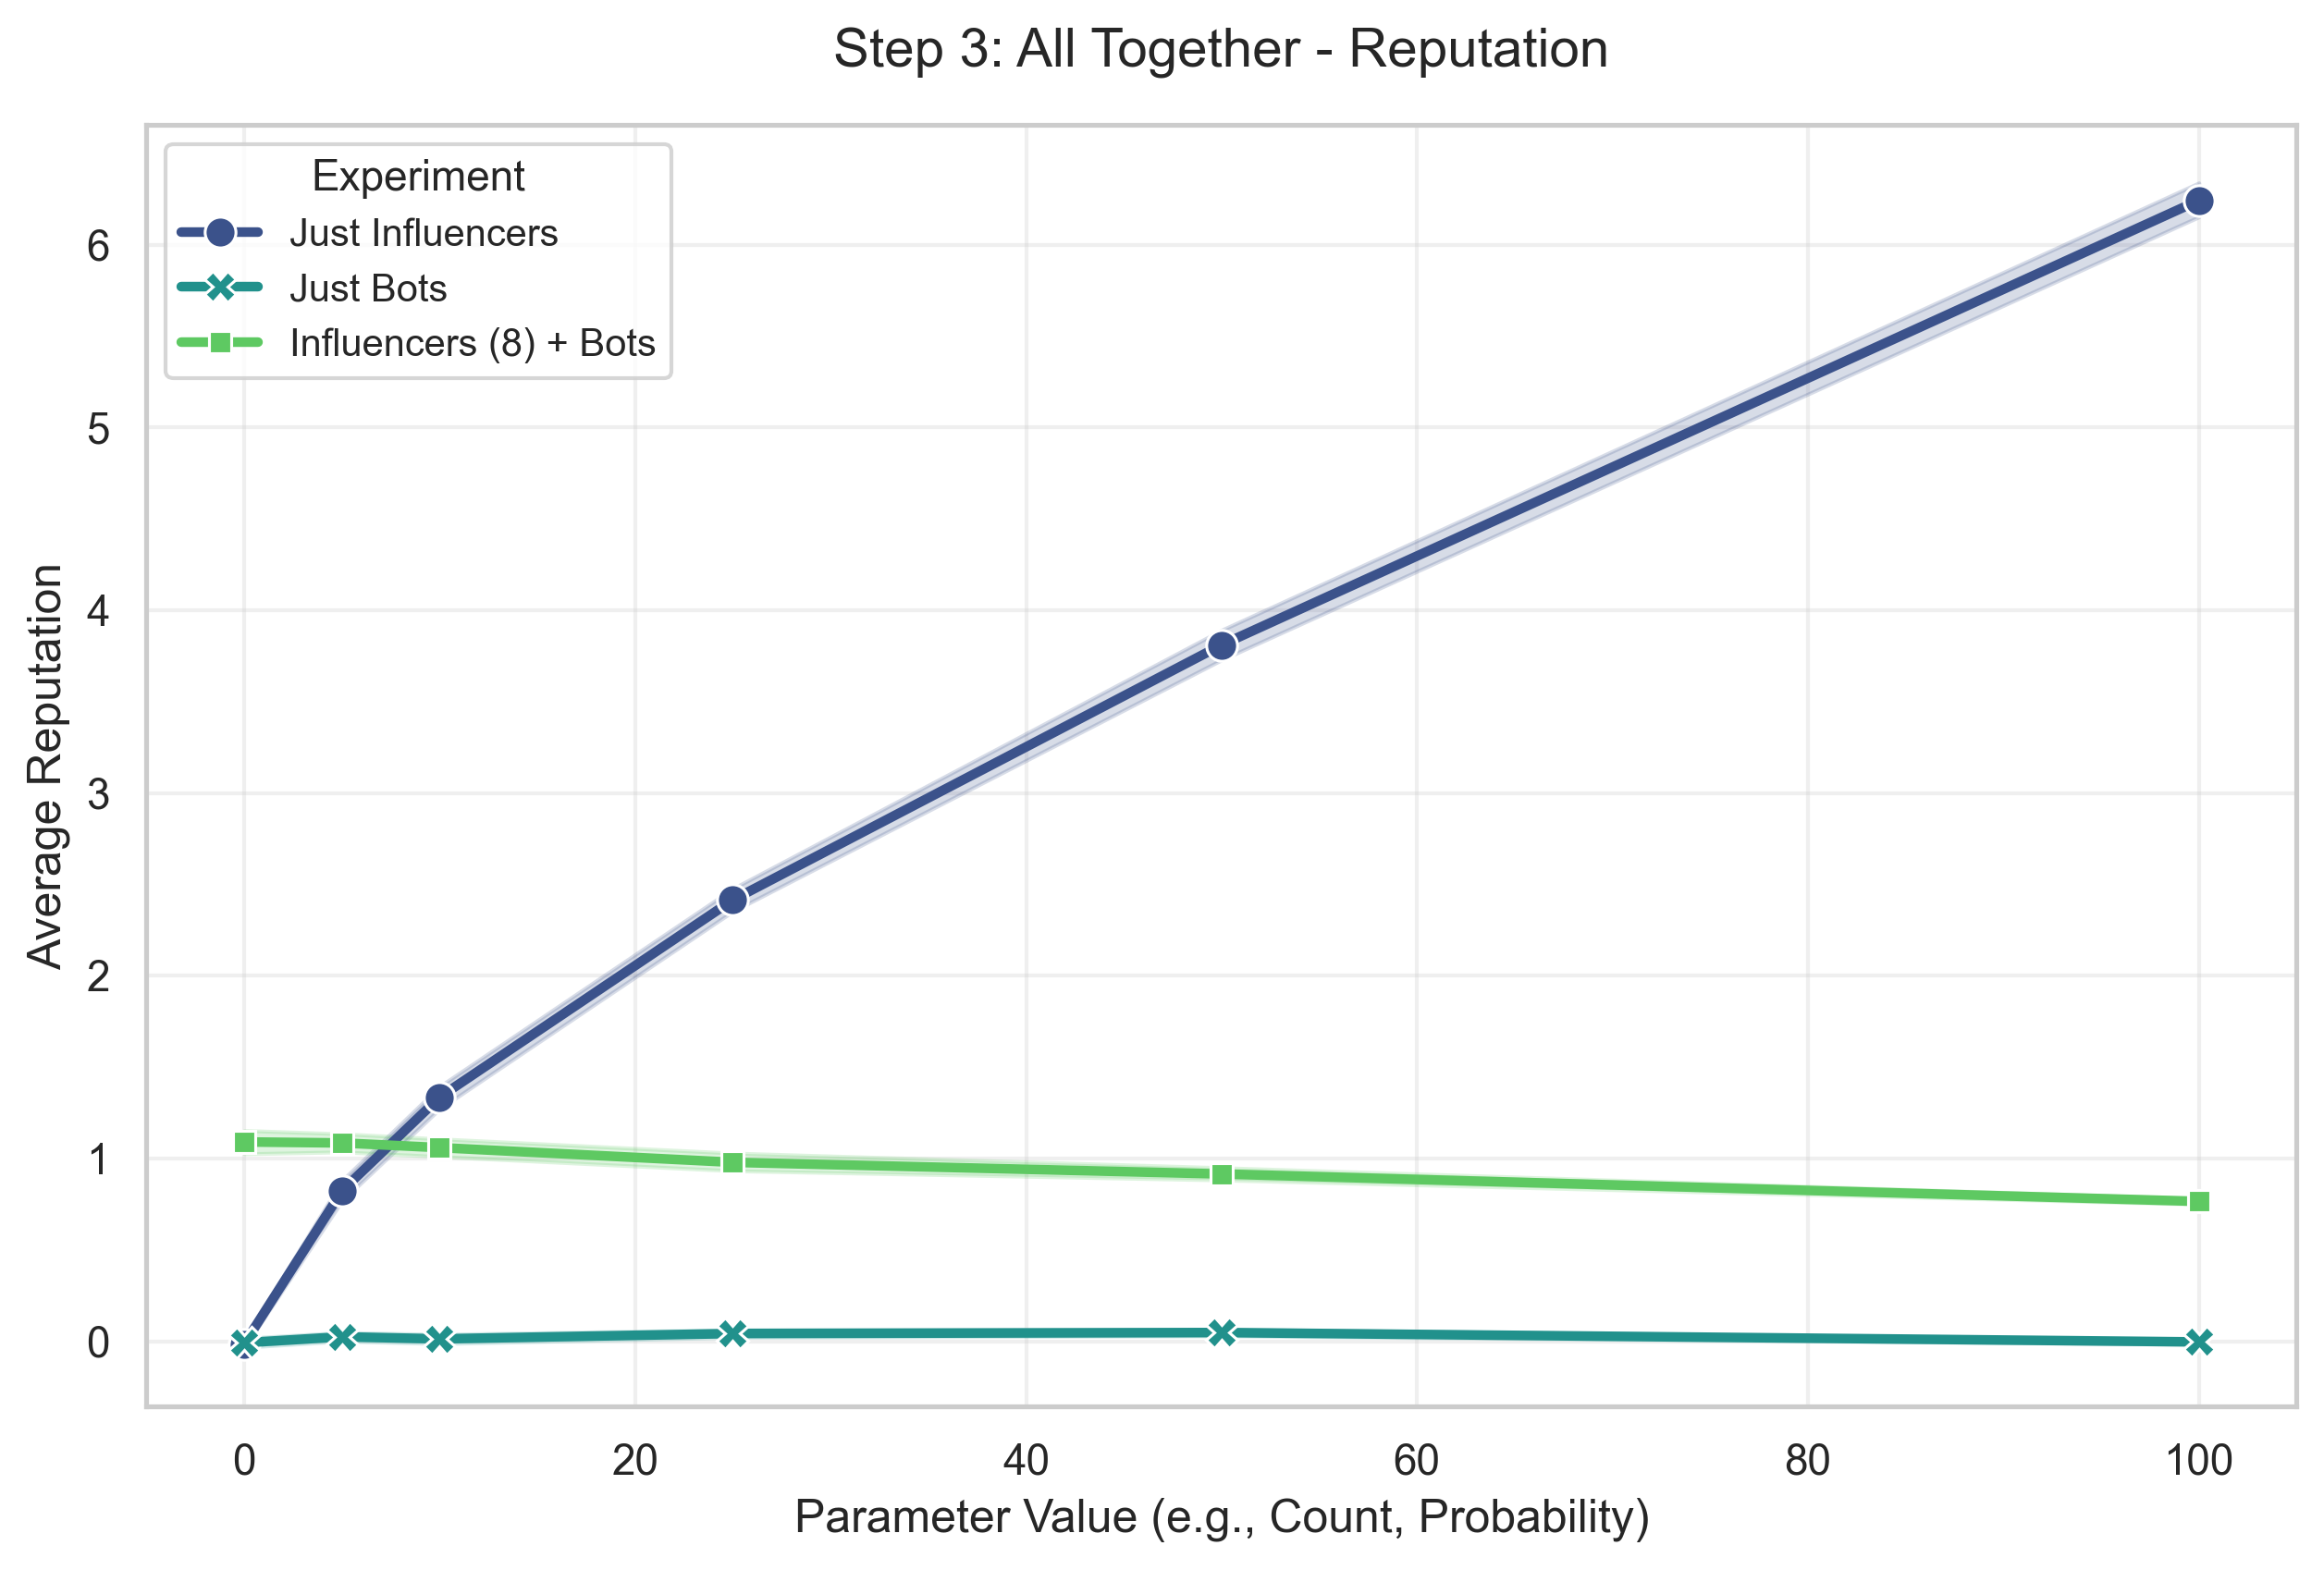
\includegraphics[width=0.8\textwidth]{figures/reputation_step3_all.png}
\caption{Reputation evolution showing the filtering mechanism: high-reputation agents maintain credibility through selective forwarding, while low-reputation agents show stable low values.}
\label{fig:reputation_step3}
\end{figure}

\subsection{Key Findings on Diffusion Patterns}

Our simulations reveal several important patterns in how this mechanism shapes misinformation spread:

\begin{enumerate}
    \item \textbf{Reputation as endogenous filter}: The penalty $\delta(\R) = \delta_0 \cdot \sigma(\R) \cdot (1 + \sigma(\R))$ is much larger for high-reputation agents, creating a feedback loop that makes them increasingly selective. This aggressive filtering significantly reduces misinformation contamination among high-reputation agents, as they require much stronger signals before forwarding.
    
    \item \textbf{Heterogeneous agent roles}: Influencers act as natural filters but can be bypassed by bots and regular users. Regular users serve as bridges between clusters, facilitating cross-community spillovers that enable misinformation to escape local containment.
    
    \item \textbf{Network amplification}: Even when reputation-sensitive agents filter effectively at the individual level, network structure can amplify spread. The presence of low-reputation agents (bots) significantly increases contamination rates, as shown in Figure~\ref{fig:misinformation_step3}.
\end{enumerate}

\begin{figure}[H]
\centering
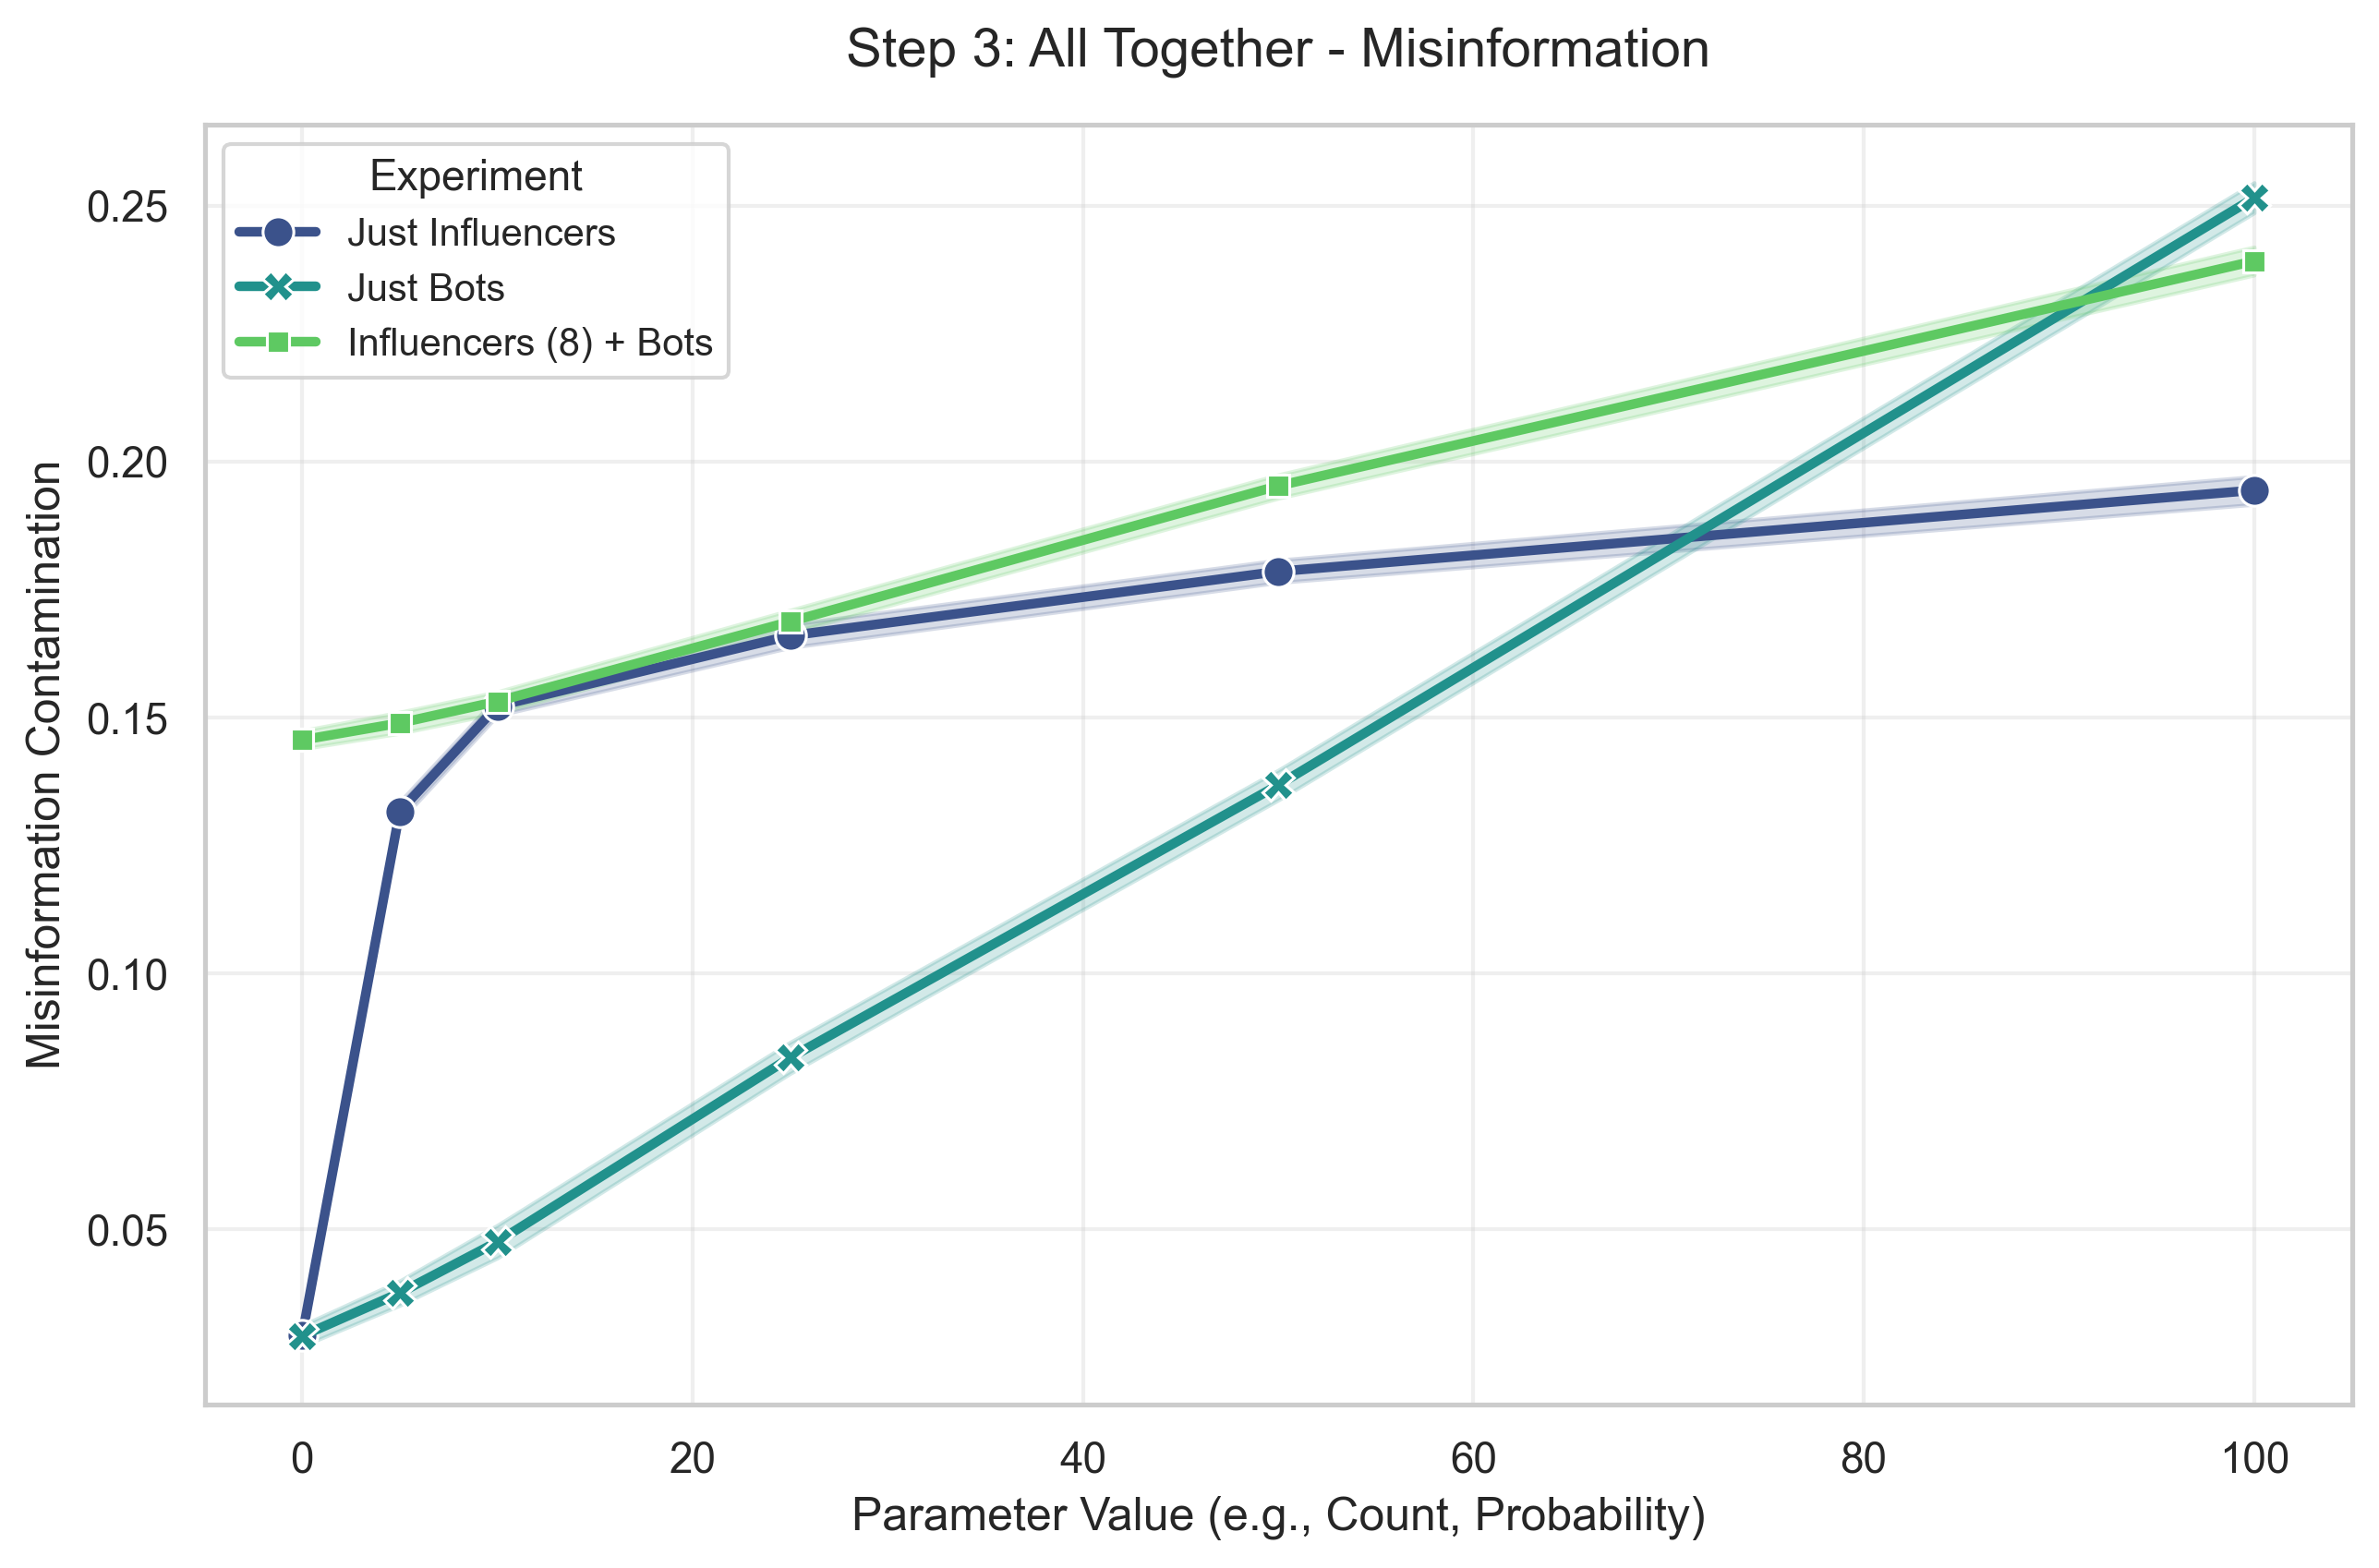
\includegraphics[width=0.8\textwidth]{figures/misinformation_step3_all.png}
\caption{Misinformation contamination patterns across agent types, showing how bots amplify spread despite filtering by high-reputation agents.}
\label{fig:misinformation_step3}
\end{figure}

Figure~\ref{fig:forwarding_step3} demonstrates the behavioral differences: influencers show lower forwarding rates due to reputation concerns, while bots forward more indiscriminately. Regular users exhibit moderate forwarding behavior, facilitating message propagation across network clusters.

\begin{figure}[H]
\centering
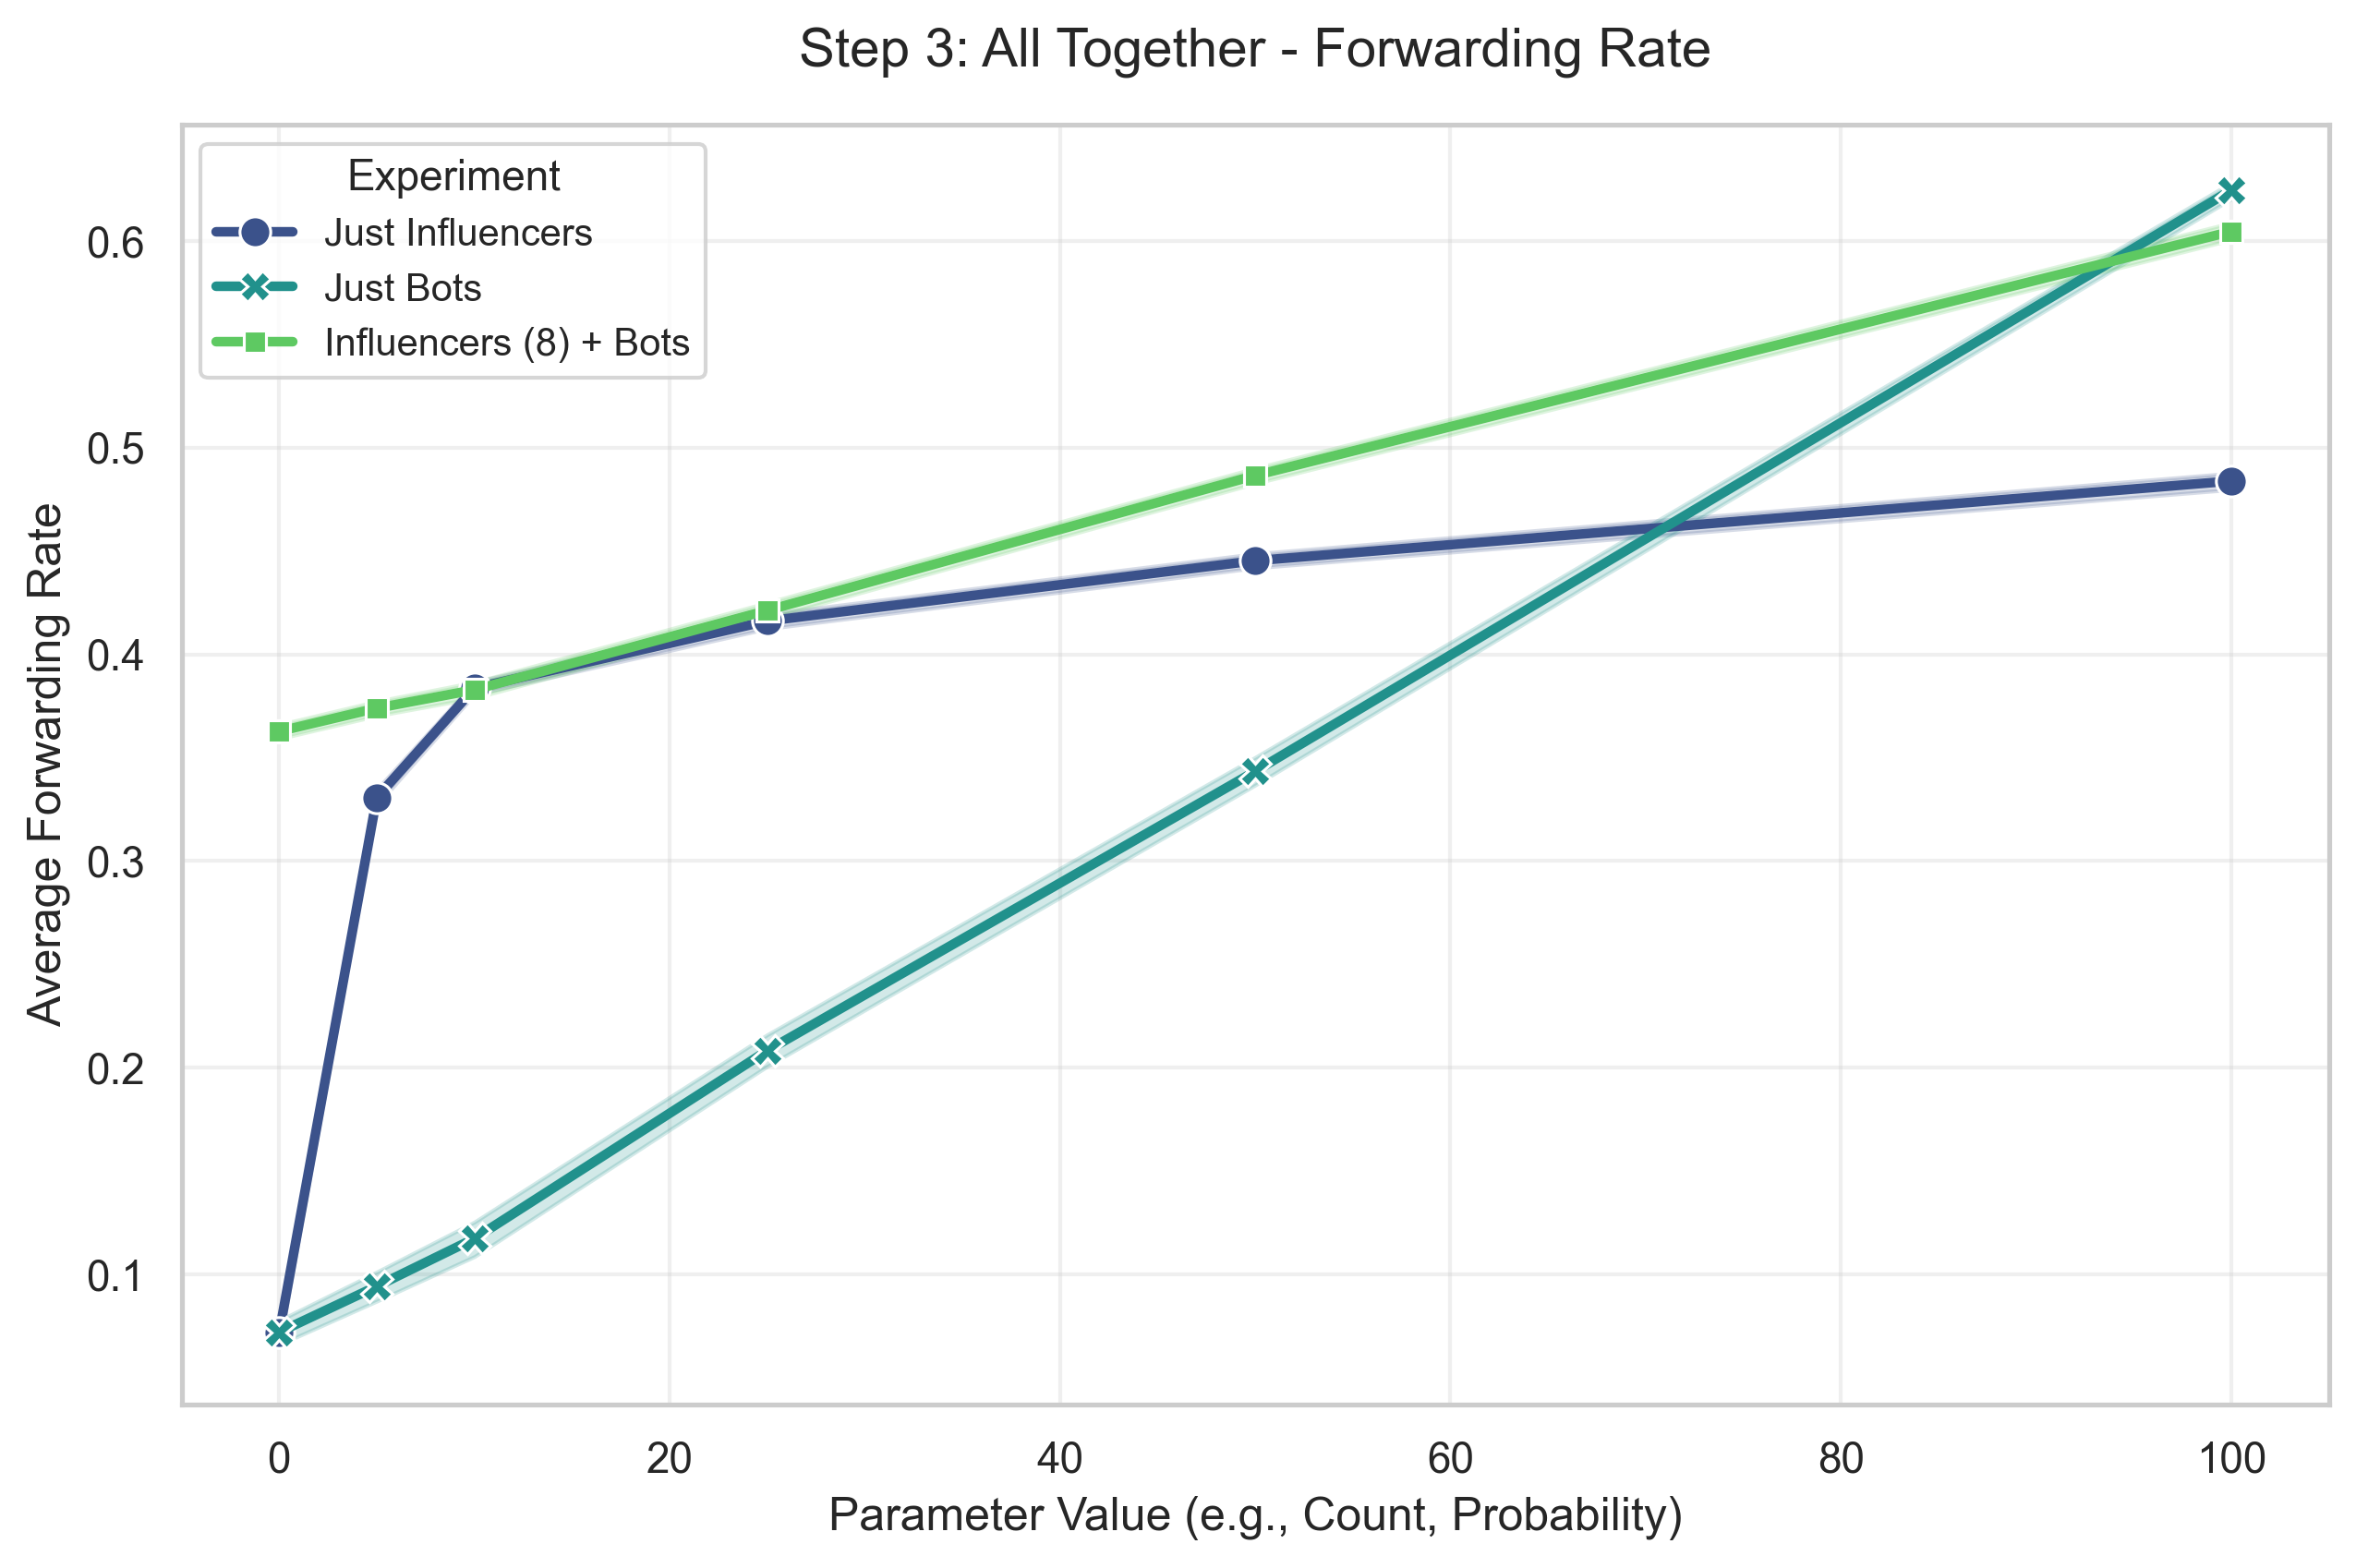
\includegraphics[width=0.8\textwidth]{figures/forwarding_step3_all.png}
\caption{Forwarding rates by agent type, illustrating how reputation sensitivity shapes forwarding decisions.}
\label{fig:forwarding_step3}
\end{figure}

\subsection{Fact-Checking Ratio and Platform Comparison}

Platforms differ significantly in their fact-checking capabilities. We abstract fact-checking as \textit{truth revelation}: after each round, the true state of the message may be revealed to agents with some probability. A higher truth-revelation probability therefore corresponds to an environment with more frequent (or more effective) fact-checking, while a lower value captures settings where verification is rare.

In our model, when truth is revealed, agents use the actual truth value $\truth$ in their utility calculation; when it is not revealed, they rely on beliefs $\widehat{\truth}$ formed from ideological proximity and sender reputation.

We compare two scenarios: (i) \textit{High fact-checking} (WhatsApp-like), where a larger fraction of messages are fact-checked and truth is observable, and (ii) \textit{Low fact-checking} (Telegram-like), where most messages lack verification and agents must rely on reputation and ideology cues.

\subsubsection{High Fact-Checking Regime (WhatsApp-like)}

When fact-checking is frequent, agents observe message truthfulness more often, which activates reputation updating more regularly. Combined with the reputation-dependent penalty $\delta(\R)$, this changes who continues to forward messages---and therefore how far messages travel (see Figures~\ref{fig:platform_reach_vs_truth_revelation_prob}--\ref{fig:platform_false_reach_count_vs_truth_revelation_prob}).

\begin{itemize}
    \item \textbf{Decreased absolute reach}: With more frequent verification, high-reputation agents become more cautious because incorrect forwarding is penalized more strongly. Since these agents typically sit in central network positions, their lower forwarding activity reduces overall reach (Figure~\ref{fig:platform_reach_vs_truth_revelation_prob}).
    
    \item \textbf{Decreased absolute false reach}: As fewer messages propagate widely, fewer agents are exposed to false messages in absolute terms (Figure~\ref{fig:platform_false_reach_count_vs_truth_revelation_prob}).
    
    \item \textbf{Increased proportional contamination}: Even as exposure falls in levels, the share of false content among messages that still circulate can rise (Figure~\ref{fig:platform_avg_misinformation_vs_truth_revelation_prob}). Intuitively, once high-reputation agents step back, diffusion is driven relatively more by low-reputation agents and bots, who face weaker penalties and are more willing to forward low-confidence content.
    
    \item \textbf{A selection channel}: The apparent paradox is therefore compositional. Stronger verification pushes the most selective (high-reputation) agents to forward less, leaving a larger role for less selective agents; this reduces false spread in absolute terms (Figure~\ref{fig:platform_false_reach_count_vs_truth_revelation_prob}), but can increase it in proportion among remaining transmissions (Figure~\ref{fig:platform_avg_misinformation_vs_truth_revelation_prob}).
\end{itemize}

\subsubsection{Low Fact-Checking Regime (Telegram-like)}

When fact-checking is rare, agents must rely primarily on reputation and ideological signals to form beliefs. This regime reveals the full force of the reputation-based mechanism:

\begin{itemize}
    \item \textbf{Higher misinformation contamination}: Without direct truth signals, agents rely more heavily on reputation and ideology, leading to higher false-forward rates. Contamination increases significantly, particularly for messages that align with agents' ideological biases (low truth-revelation probabilities in Figure~\ref{fig:platform_avg_misinformation_vs_truth_revelation_prob}).
    
    \item \textbf{Strengthened reputation premium}: The reputation mechanism becomes more powerful when verification is scarce. High-reputation agents gain a larger advantage because their reputation serves as a crucial signal for other agents, increasing reputation inequality across agent types (consistent with the mechanism in Figure~\ref{fig:reputation_step3}).
    
    \item \textbf{Ideological echo chambers}: With limited fact-checking, ideological alignment becomes a primary belief signal. Messages aligned with agents' biases are more likely to be forwarded, even when false, creating stronger echo-chamber dynamics (low truth-revelation probabilities in Figures~\ref{fig:platform_reach_vs_truth_revelation_prob} and~\ref{fig:platform_avg_misinformation_vs_truth_revelation_prob}).
\end{itemize}

\subsubsection{Comparative Impact}

The comparison highlights a key policy implication: fact-checking does not only change beliefs; it also reshapes diffusion by shifting who remains active in forwarding.

In high fact-checking environments (WhatsApp), more frequent verification activates reputation penalties more often, making high-reputation agents markedly more selective. Because these agents have outsized network influence, their withdrawal reduces overall reach and lowers false reach in absolute terms. At the same time, the messages that continue to circulate are disproportionately carried by less selective agents, which can raise the proportional contamination rate.

In low fact-checking environments (Telegram), verification is scarce and reputation becomes the main credibility cue. High-reputation agents still filter, but because the truth is revealed less often, the reputational consequences are triggered less frequently and selectivity is weaker than under high fact-checking. This creates room for low-reputation agents (especially bots) to sustain diffusion of false content, raising absolute contamination.

Overall, fact-checking and reputation-based filtering interact through an endogenous selection mechanism: stronger verification increases the effective penalty borne by high-reputation agents, reducing their forwarding activity, which lowers false exposure in levels but can concentrate misinformation among the remaining diffusion paths. Finally, the magnitude of any reduction in false-message spread---especially when measured in percentages---depends critically on the prevalence of bots (agents who share regardless of truthfulness): reducing the number of bots mechanically strengthens the decline in false reach.

\subsubsection{Platform Comparison under Varying Fact-Checking}

To make the platform comparison more transparent, we vary the probability that message truthfulness is revealed to agents after each round (the truth-revelation probability), spanning Telegram-like (low fact-checking) to WhatsApp-like (high fact-checking). We report three complementary reach measures: overall reach, false reach as a share of the network, and false reach in absolute counts. Together, these figures highlight the selection channel discussed above: total exposure can fall while proportional contamination rises.

\begin{figure}[H]
\centering
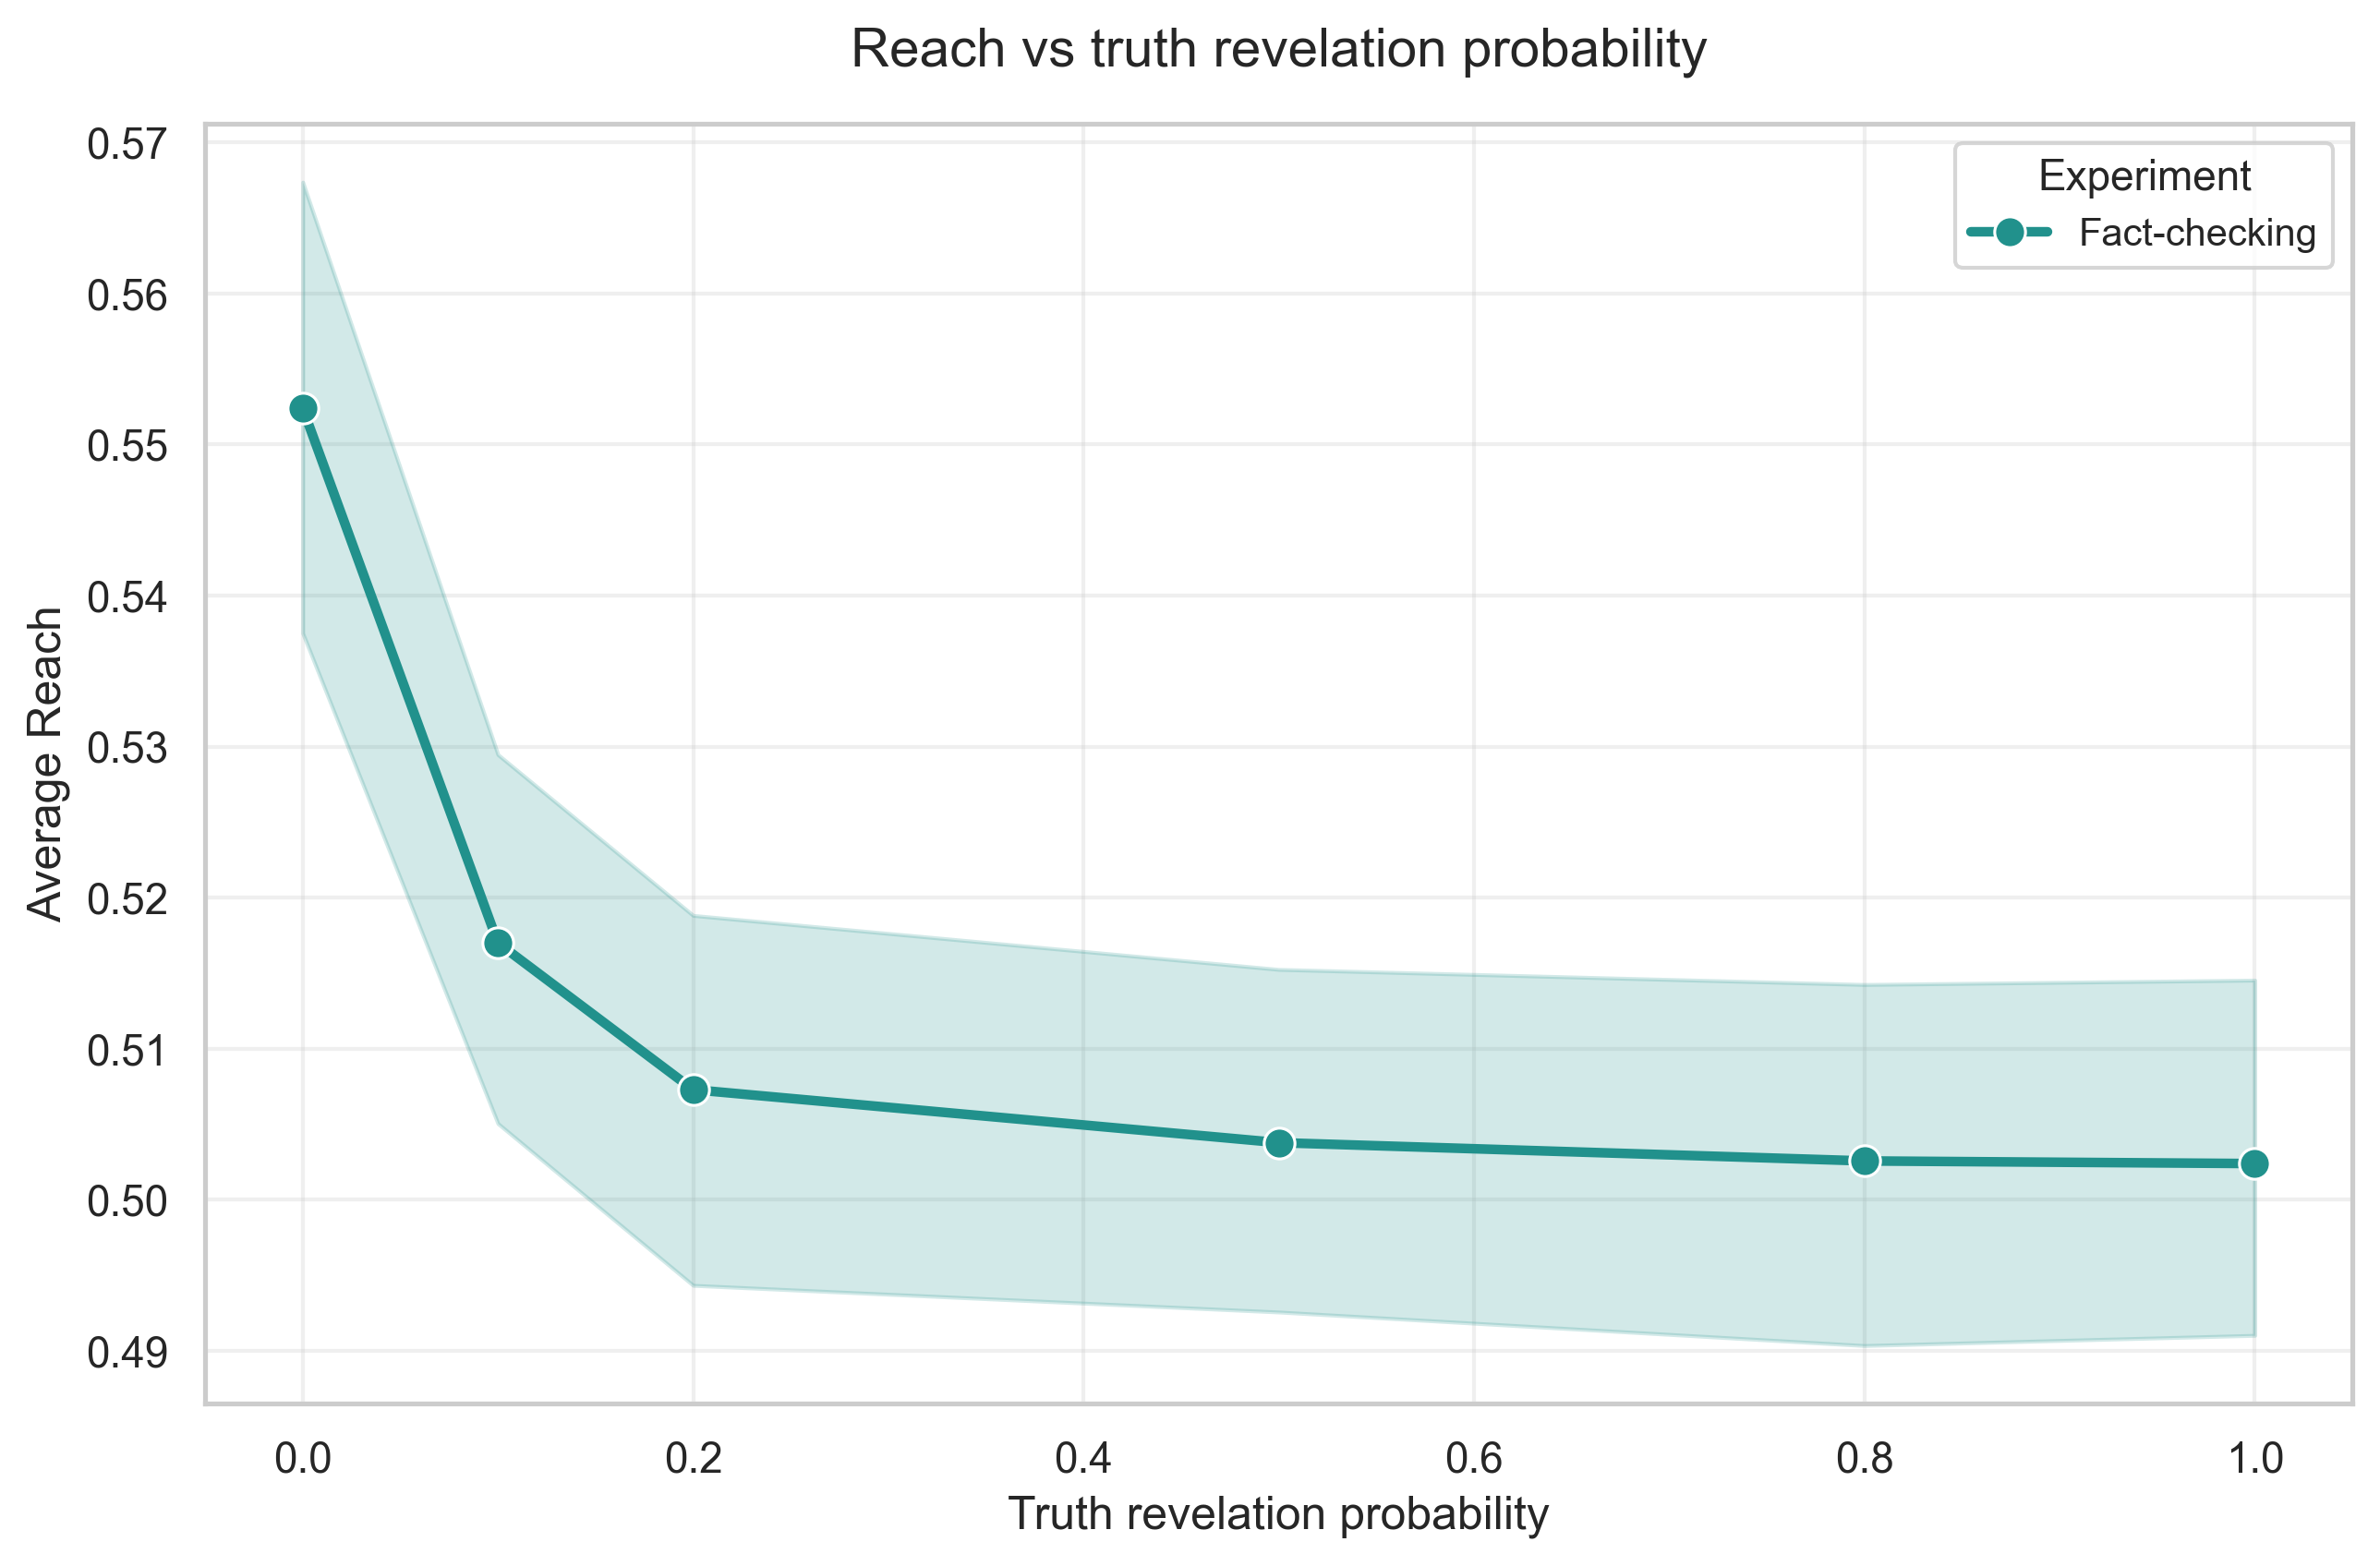
\includegraphics[width=0.9\textwidth]{figures/platform_reach_vs_truth_revelation_prob.png}
\caption{Overall message reach as the truth-revelation probability varies (low values are Telegram-like; high values are WhatsApp-like).}
\label{fig:platform_reach_vs_truth_revelation_prob}
\end{figure}

\begin{figure}[H]
    \centering
    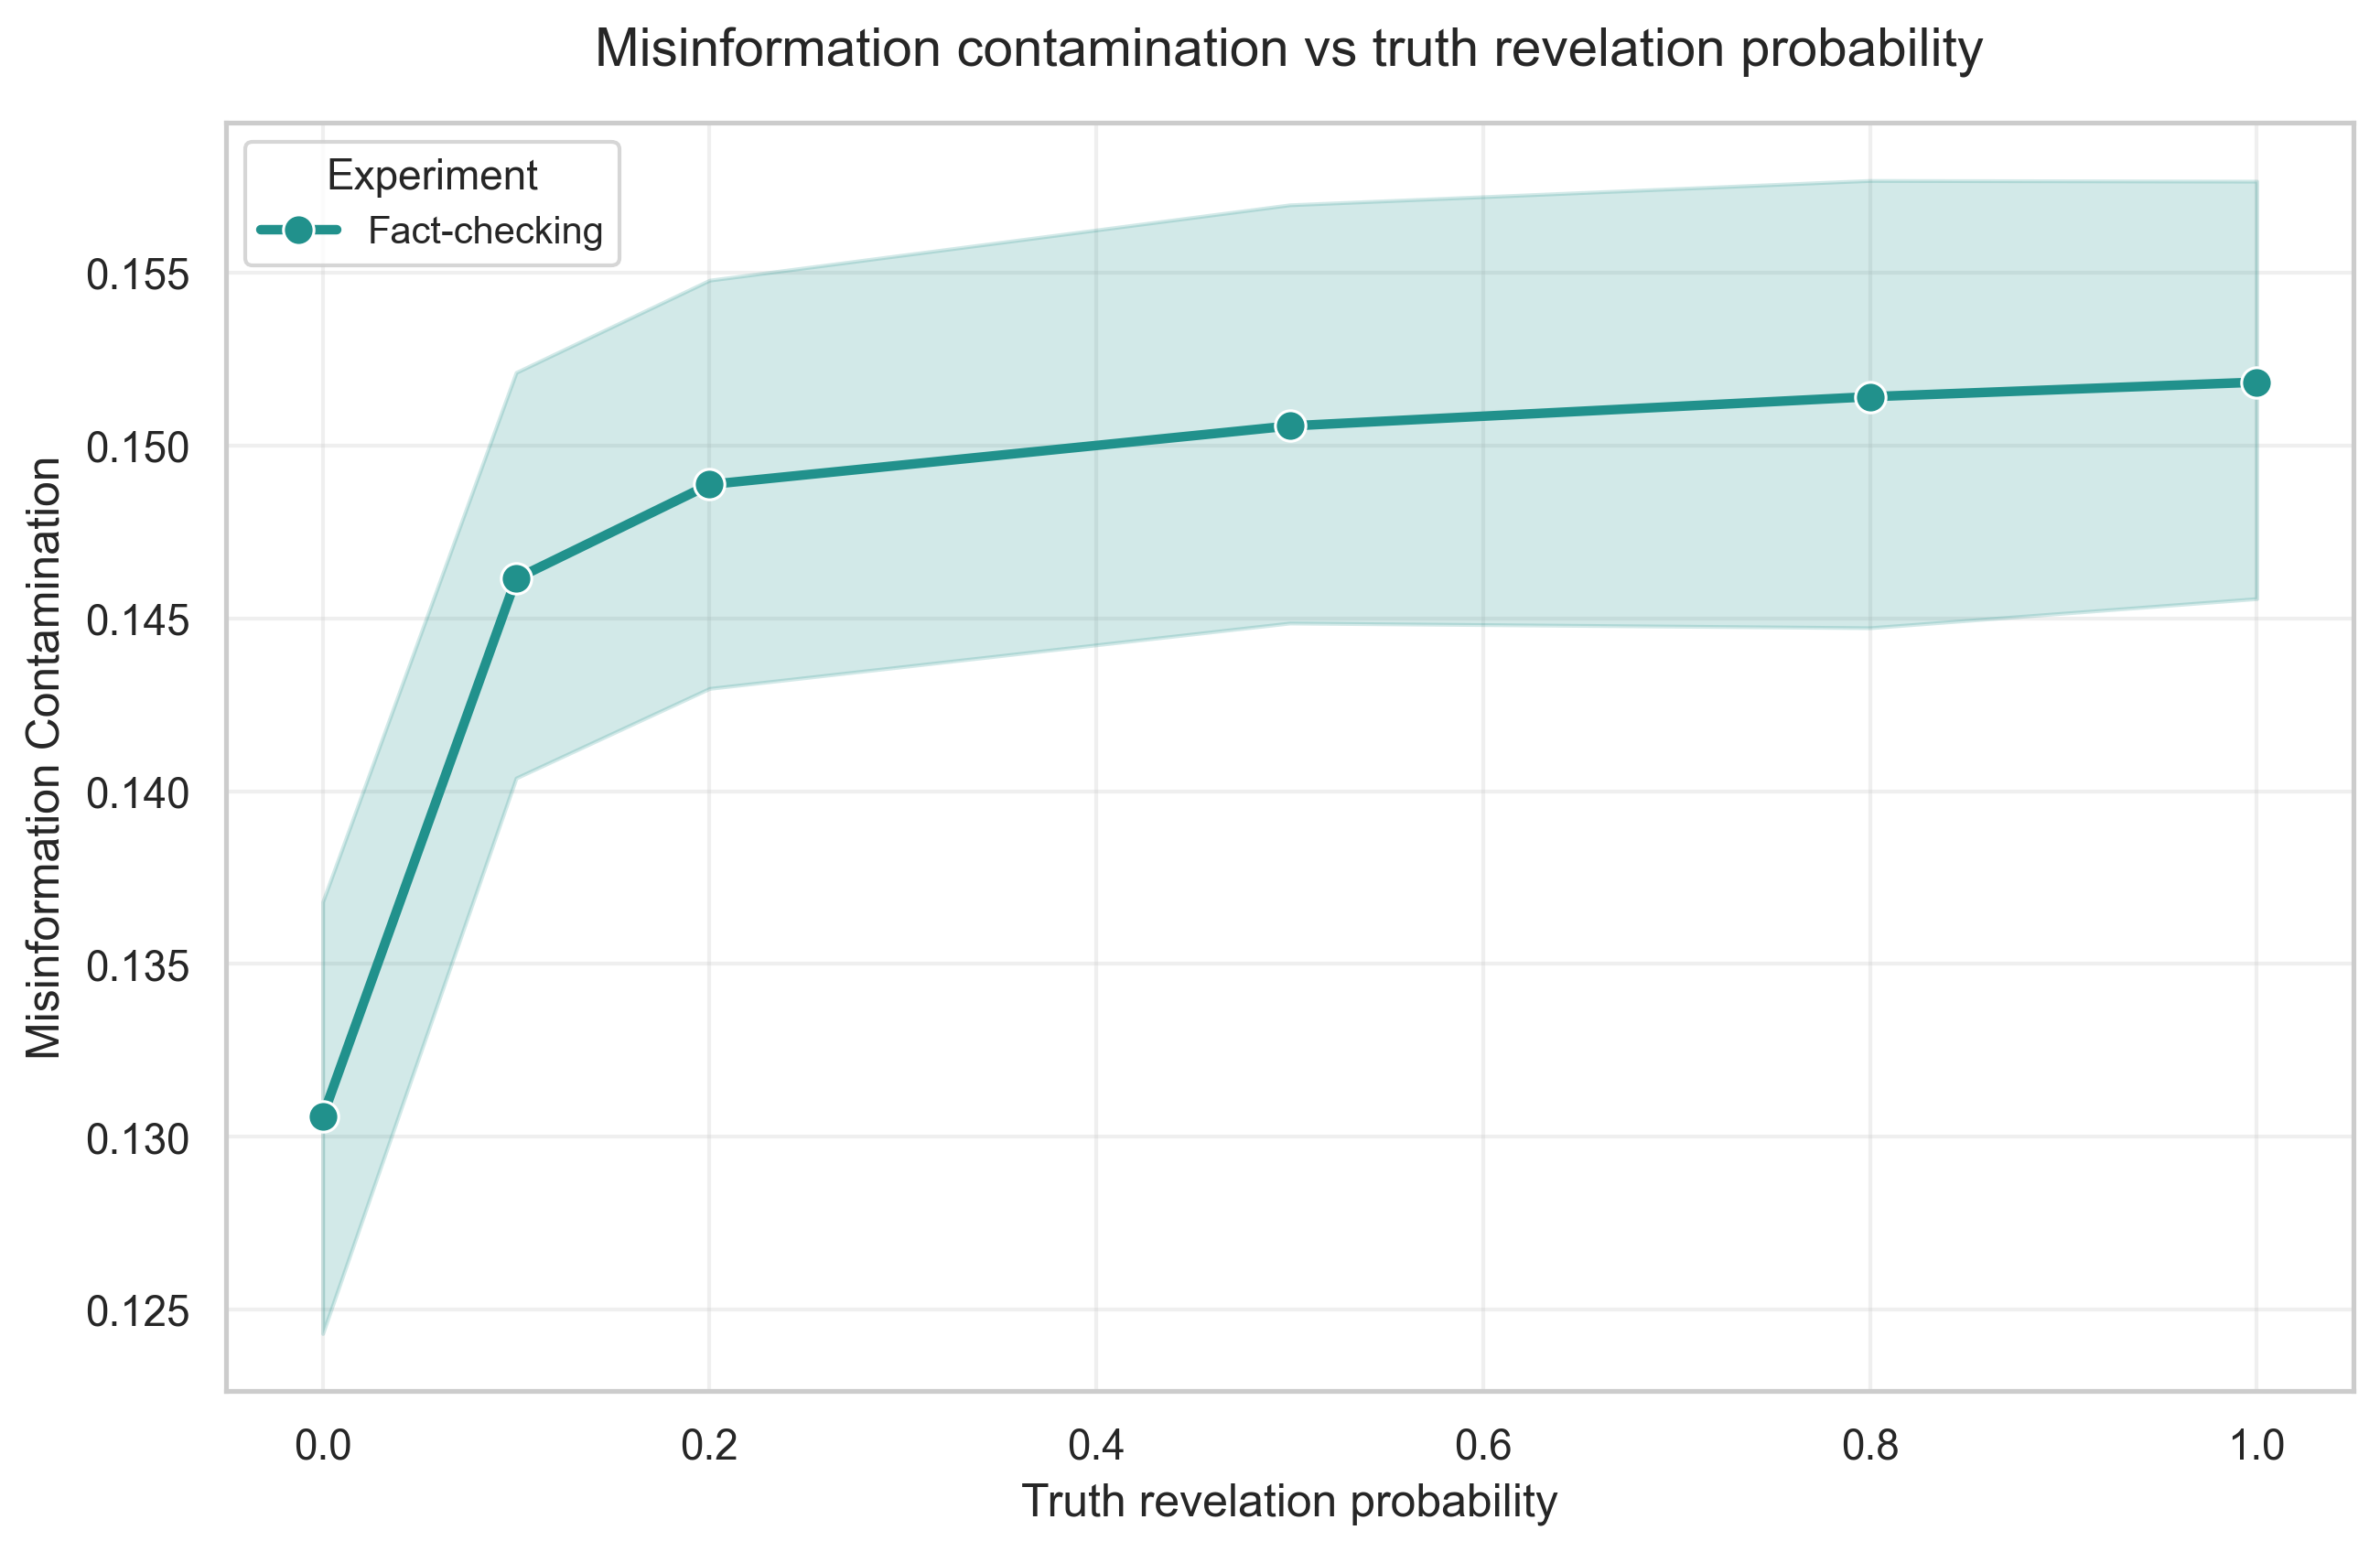
\includegraphics[width=0.9\textwidth]{figures/platform_avg_misinformation_vs_truth_revelation_prob.png}
    \caption{Misinformation contamination (proportion) as the truth-revelation probability varies.}
    \label{fig:platform_avg_misinformation_vs_truth_revelation_prob}
\end{figure}

\begin{figure}[H]
\centering
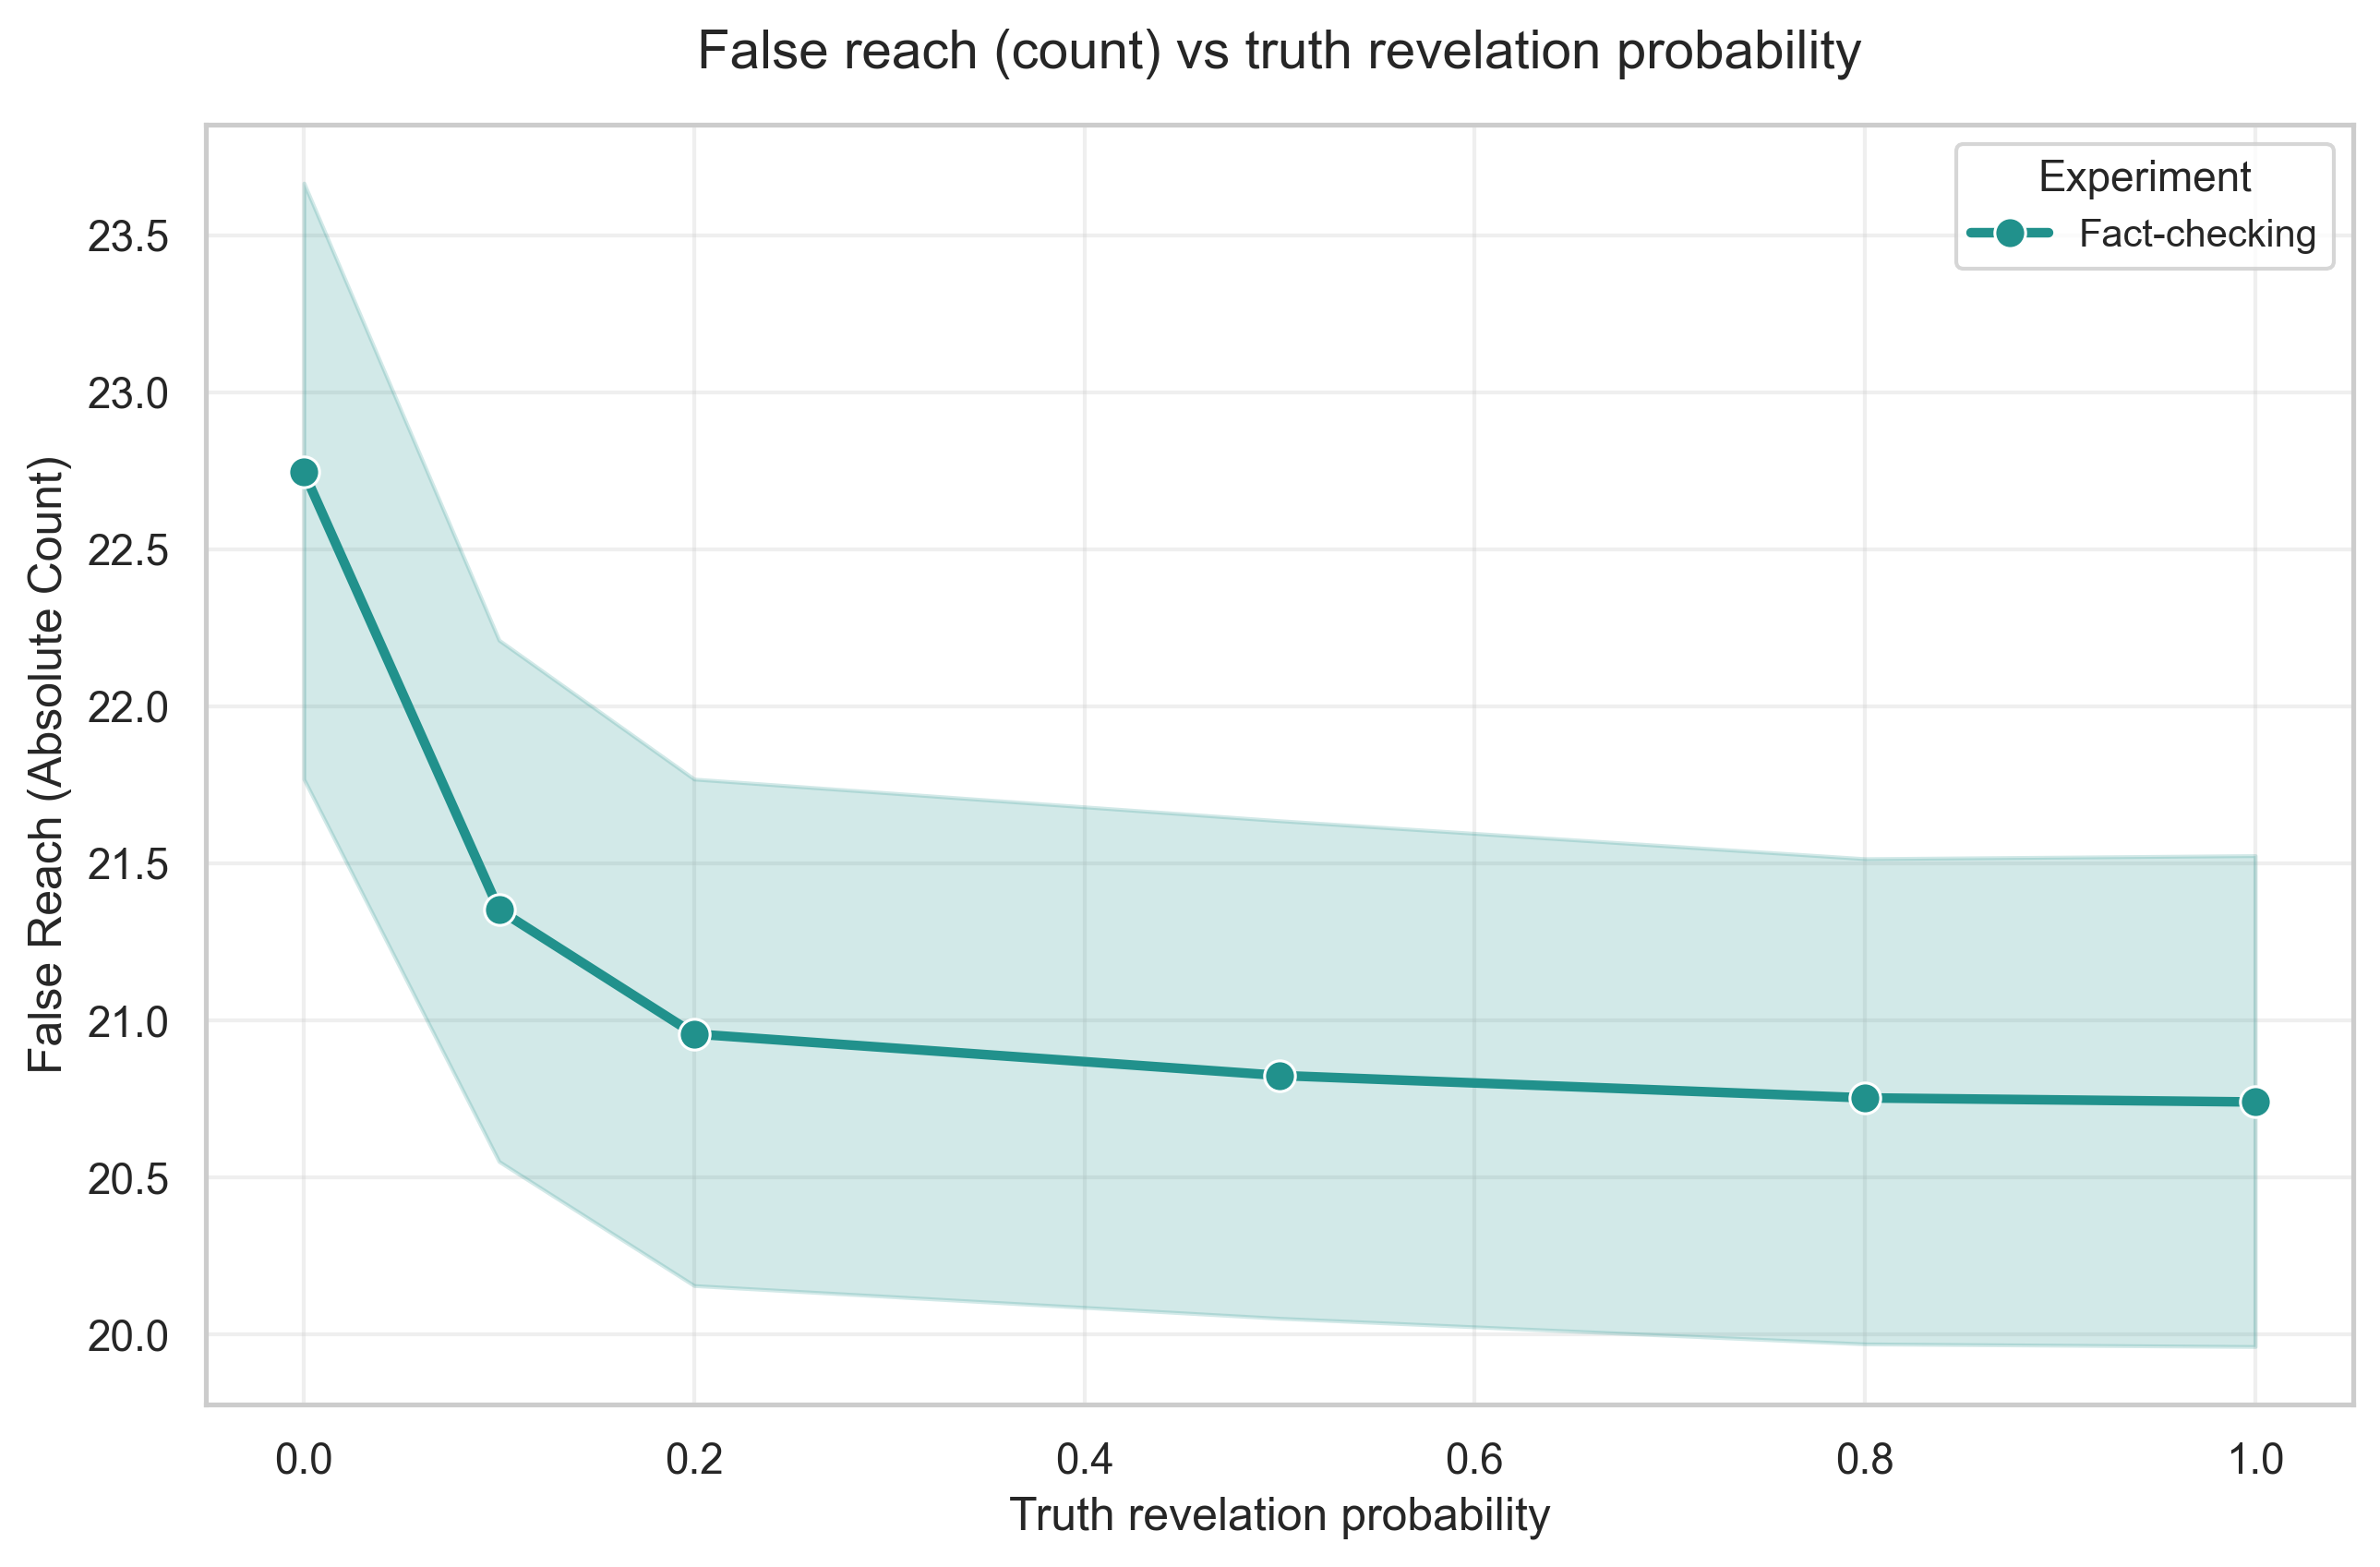
\includegraphics[width=0.9\textwidth]{figures/platform_false_reach_count_vs_truth_revelation_prob.png}
\caption{False reach (absolute number of agents exposed to false messages) as the truth-revelation probability varies.}
\label{fig:platform_false_reach_count_vs_truth_revelation_prob}
\end{figure}

\subsubsection{Bots and False-Message Spread in Telegram-like Environments}

Finally, focusing on the Telegram-like setting, we vary the number of bots and examine how false-message spread changes. Because bots forward largely irrespective of truthfulness, reductions in bots are a key driver of reductions in false spread---including when measured in percentages.

\begin{figure}[H]
\centering
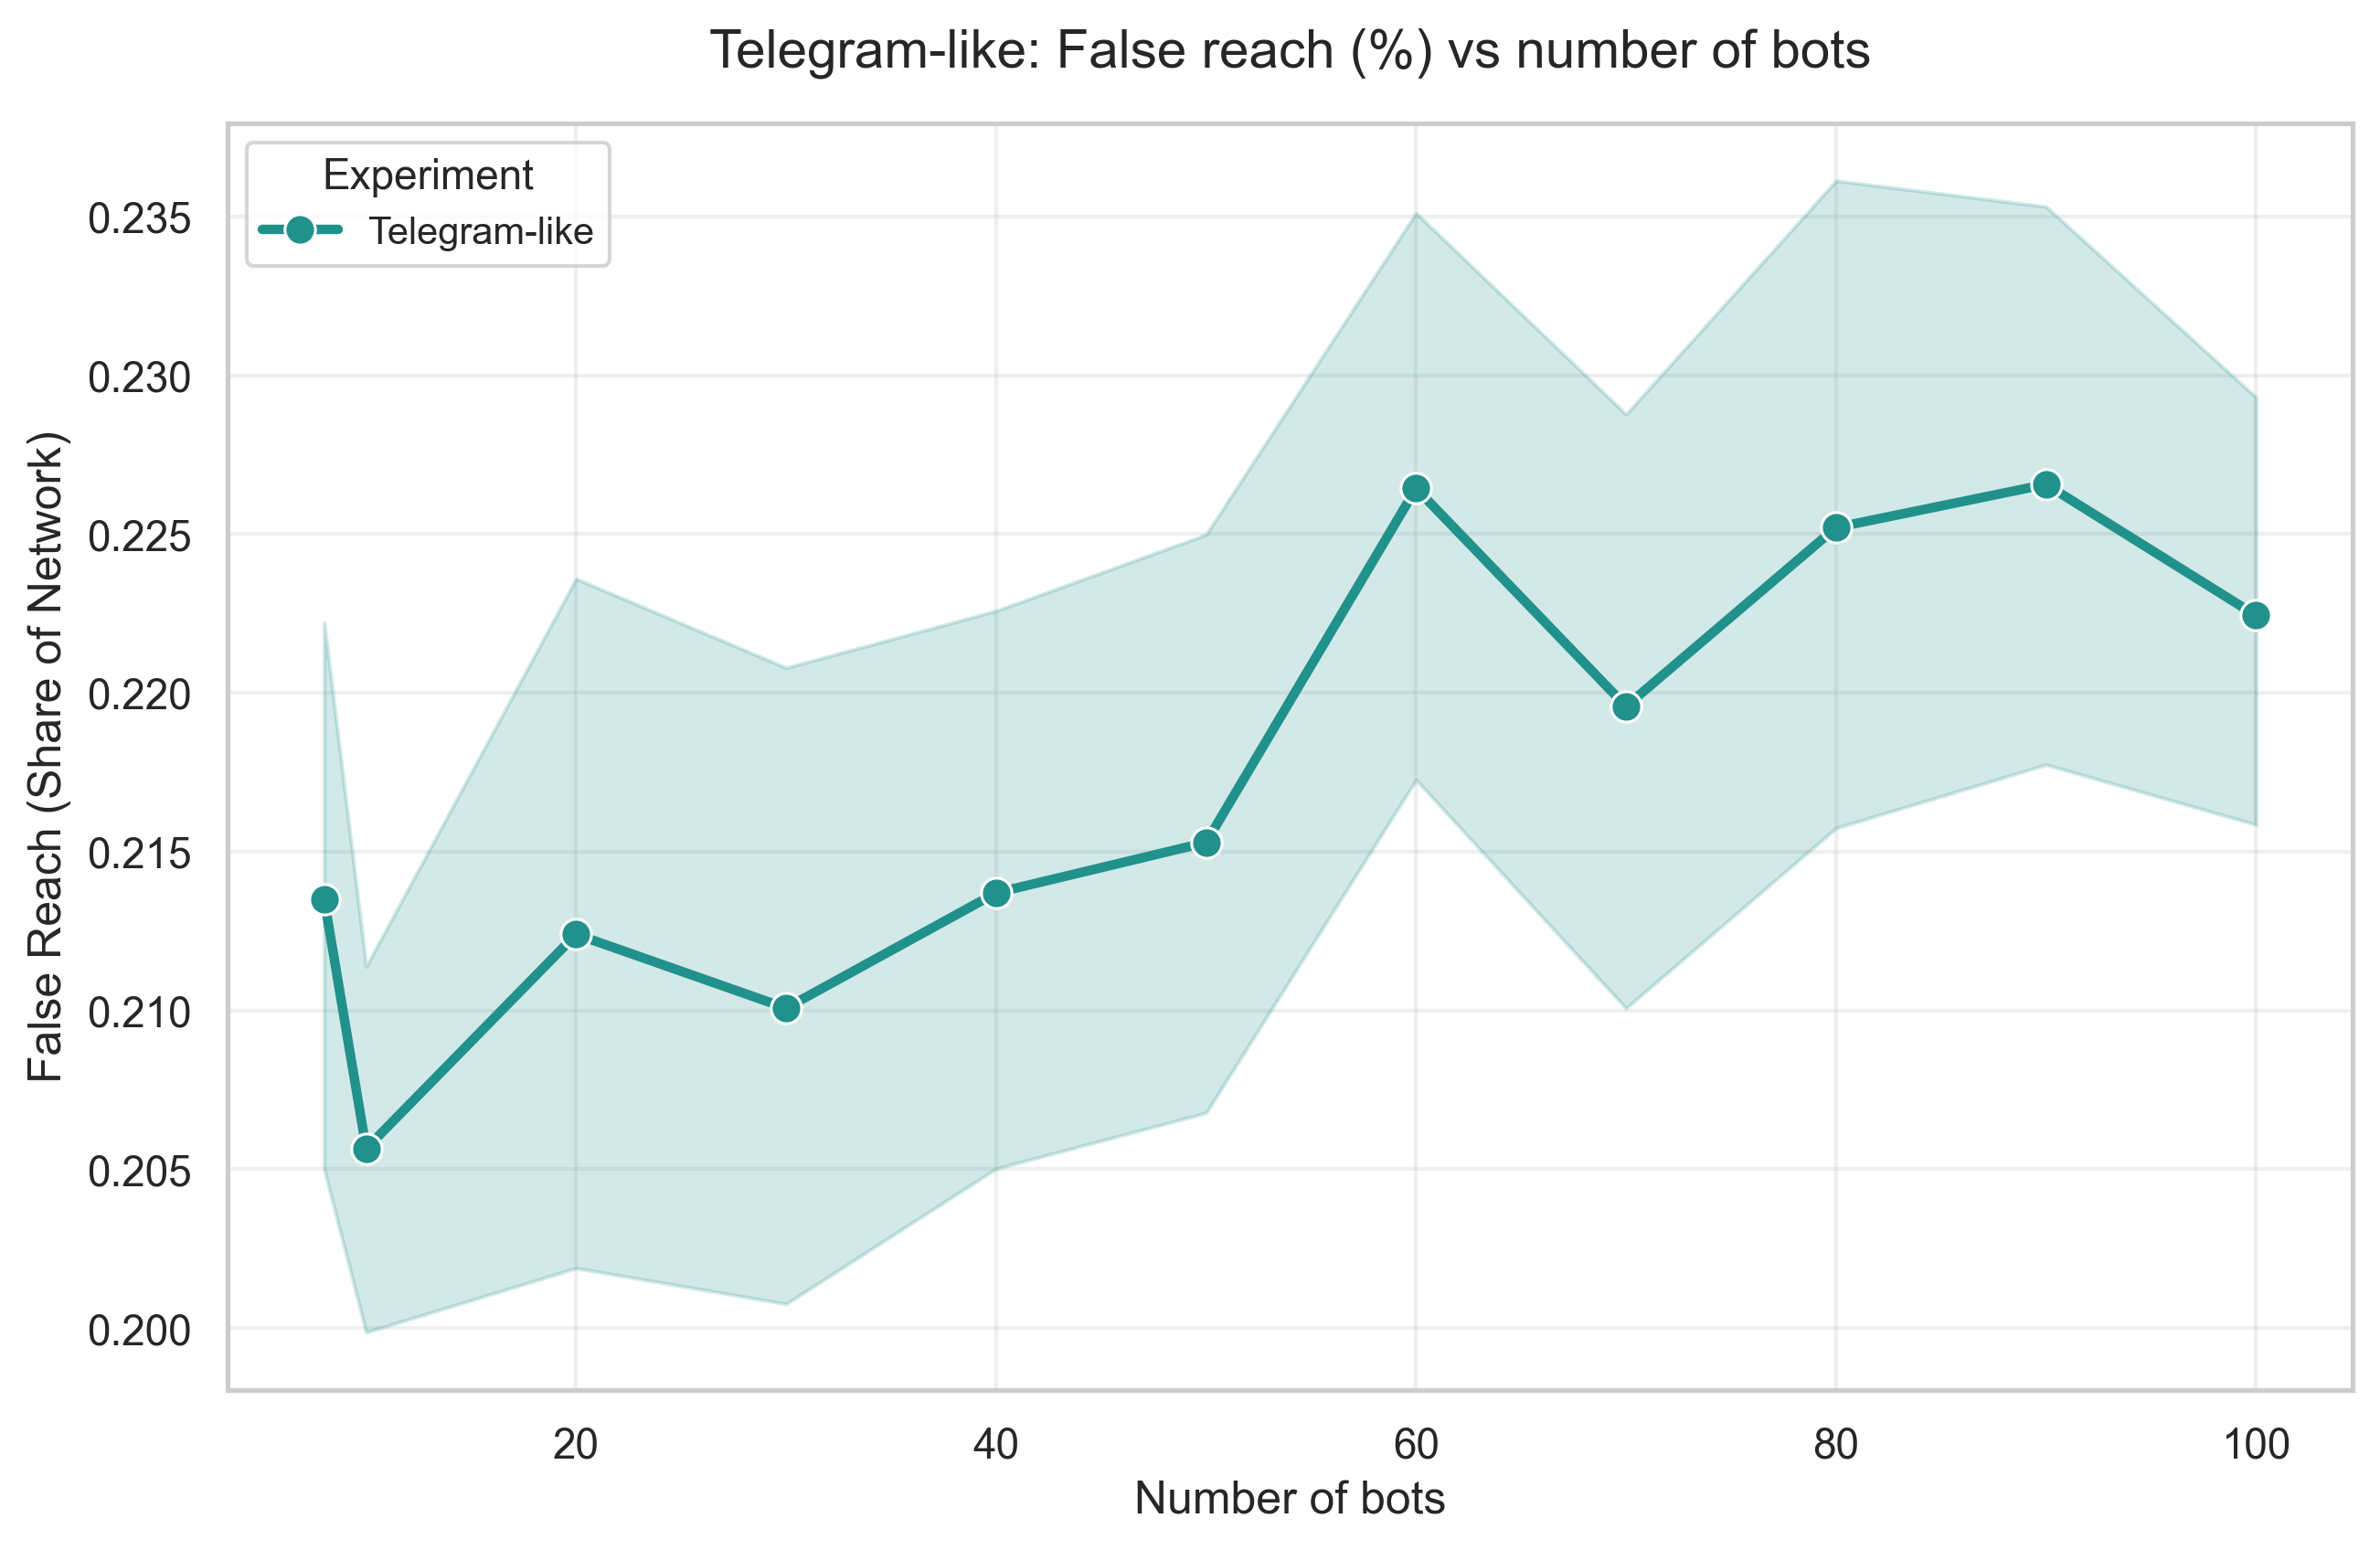
\includegraphics[width=0.9\textwidth]{figures/telegram_false_spread_vs_bots.png}
\caption{Telegram-like environment: false-message spread (percentage) as the number of bots varies.}
\label{fig:telegram_false_spread_vs_bots}
\end{figure}

\begin{figure}[H]
\centering
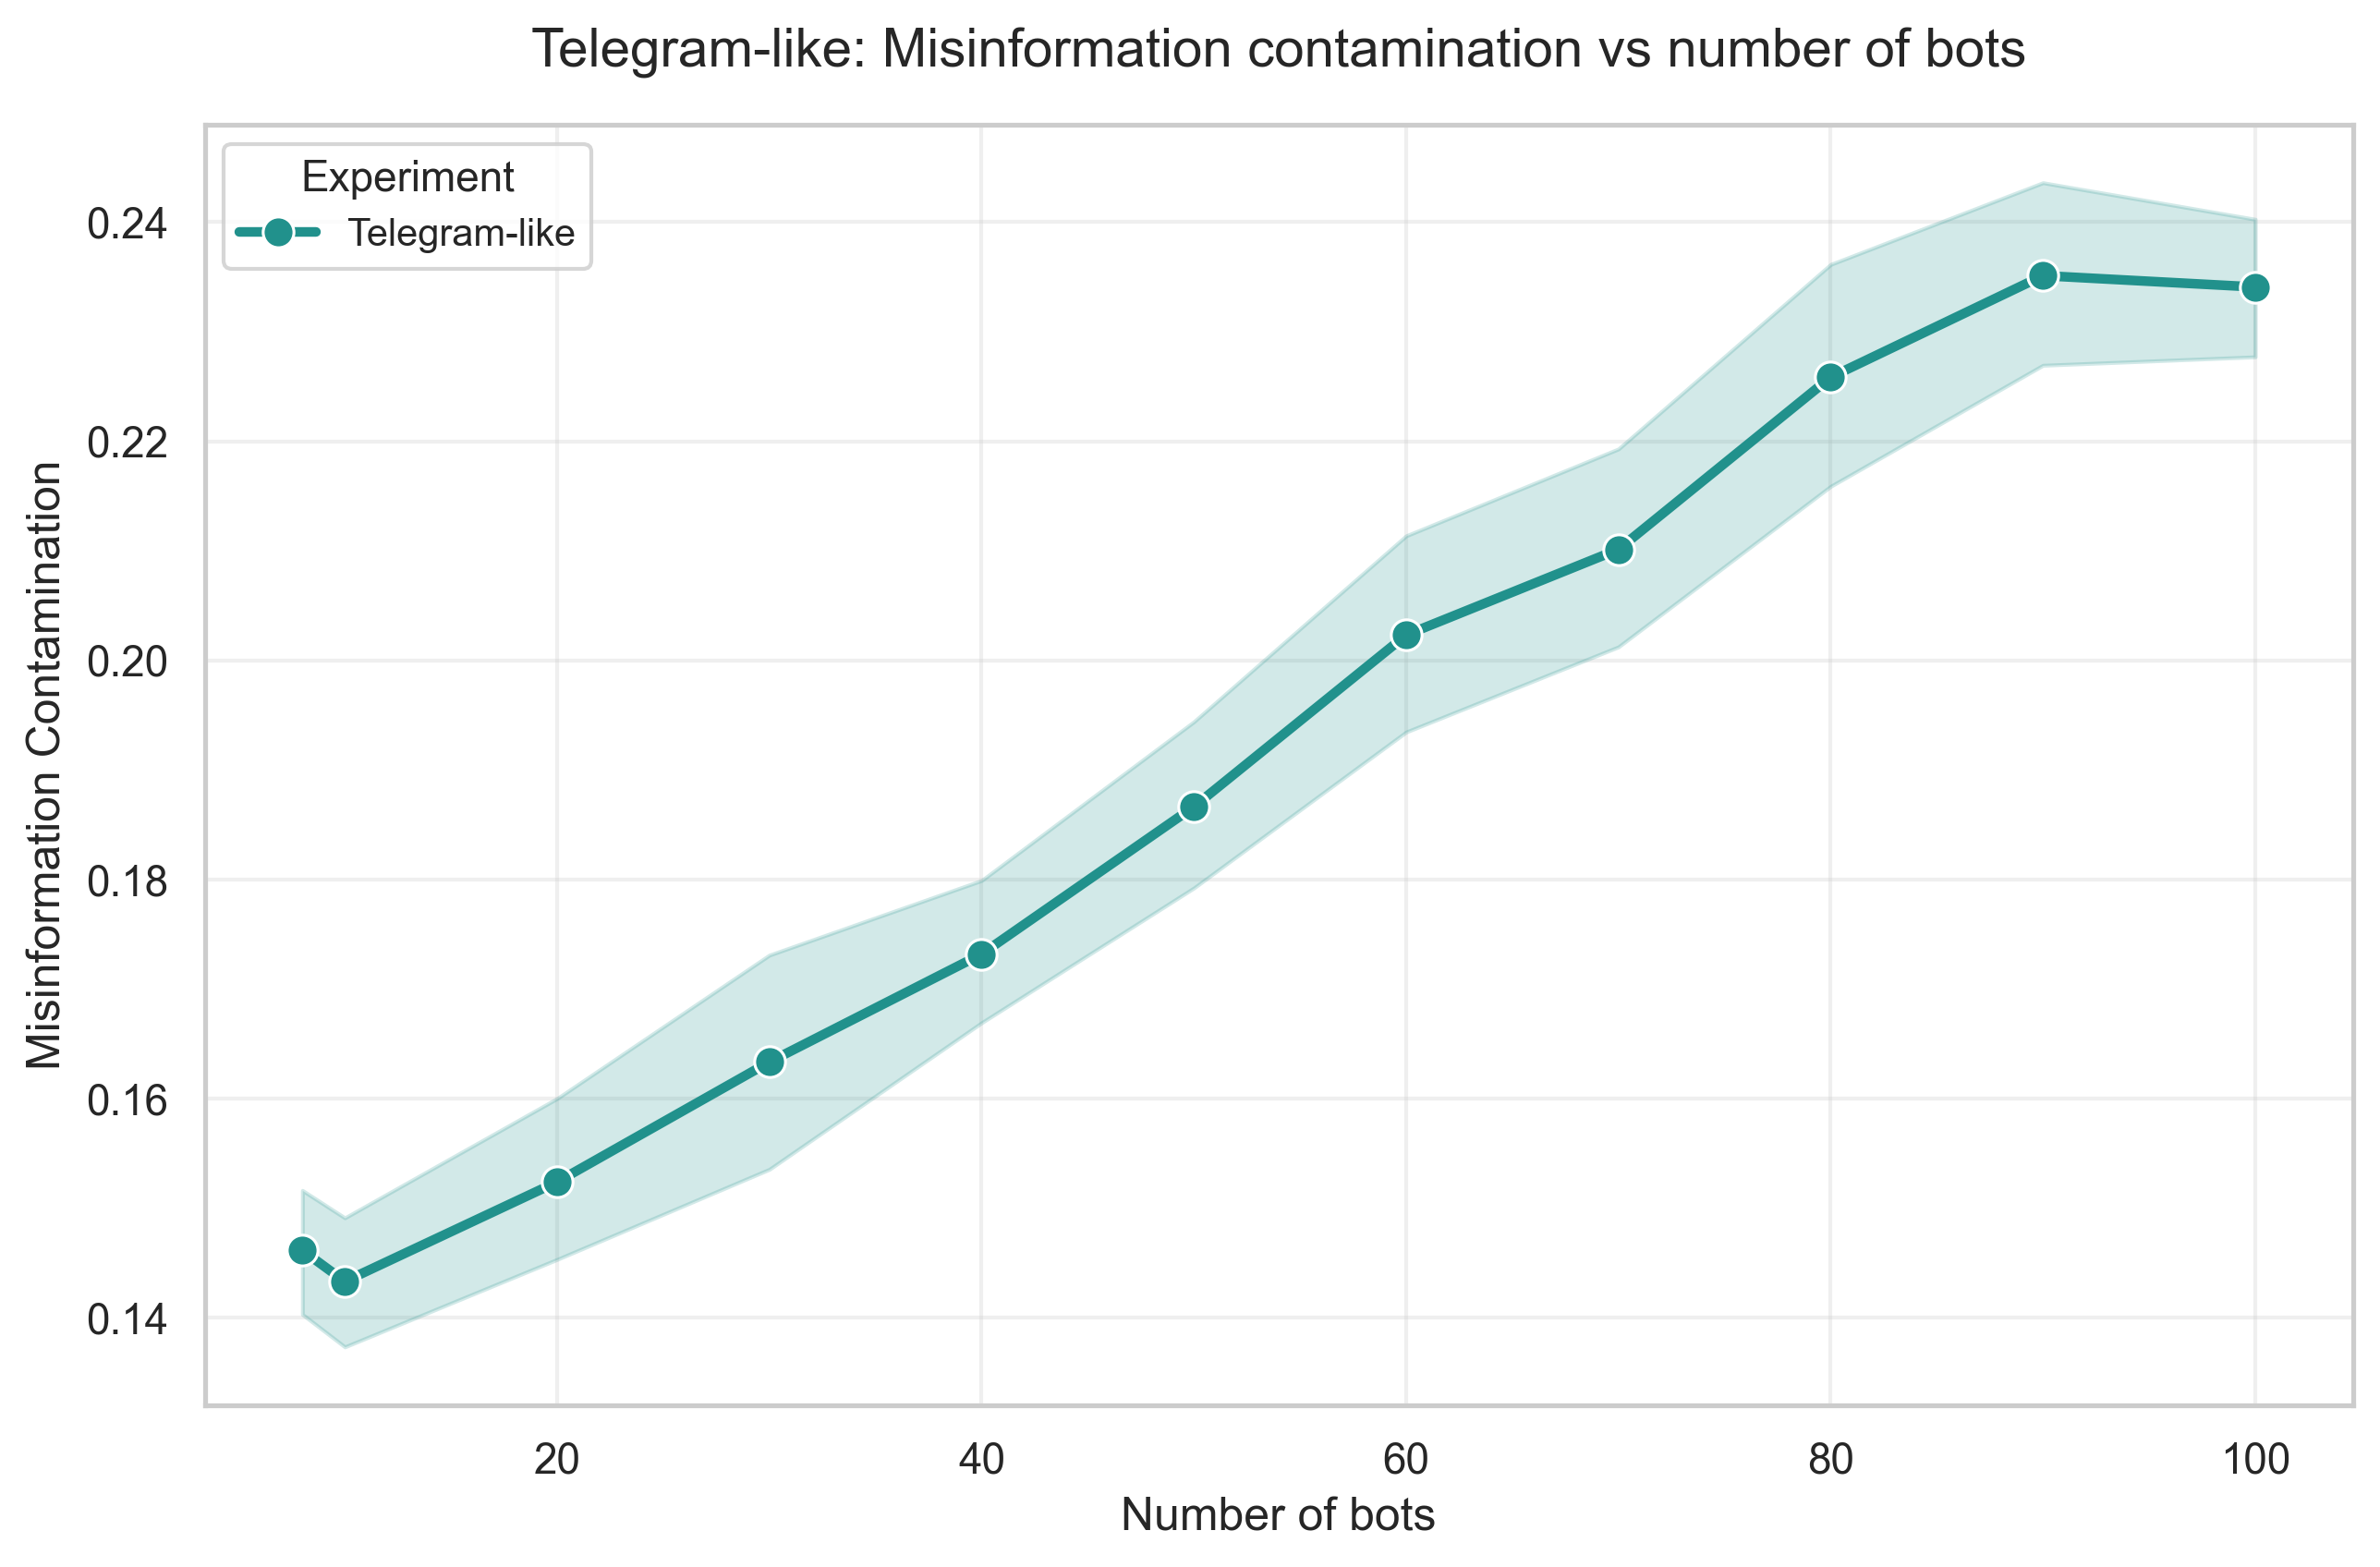
\includegraphics[width=0.9\textwidth]{figures/telegram_avg_misinformation_vs_bots.png}
\caption{Telegram-like environment: misinformation contamination (proportion) as the number of bots varies.}
\label{fig:telegram_avg_misinformation_vs_bots}
\end{figure}


\section{Conclusion}
\subsection{Conclusion}

This paper studies misinformation diffusion in a WhatsApp/Telegram-like environment where agents decide whether to forward messages based on ideological proximity and reputational incentives. The key mechanism is an endogenous reputational filter: agents with higher reputation face stronger expected losses from forwarding false content and therefore become more selective over time, while low-reputation agents (and especially bots) remain comparatively willing to share.

Our simulation results highlight a central selection effect in platform-level fact-checking. When we increase the truth-revelation probability (our abstraction of more frequent or more effective fact-checking), high-reputation agents become more cautious and reduce their forwarding activity. Because these agents typically occupy influential network positions, this lowers overall reach and reduces false-message exposure in absolute terms (false reach in counts). At the same time, misinformation can become more concentrated among the messages that still circulate, since diffusion is increasingly carried by less selective agents and bots. In other words, stronger fact-checking can simultaneously reduce the level of false exposure while increasing the proportion of misinformation among remaining transmissions.

Finally, varying the number of bots shows that bots are a first-order determinant of false-message spread. Because bots forward largely regardless of truthfulness, reducing their prevalence mechanically strengthens the decline in false reach and improves percentage-based misinformation outcomes. This reinforces a practical policy implication: platform interventions that limit automated or indiscriminate forwarding can complement fact-checking by weakening the main channel through which false content continues to propagate when selective agents disengage.

\subsection{Model Limitations}

Several simplifying assumptions constrain the realism of the simulation:

\begin{itemize}
    \item \textbf{Ideological bias is one-dimensional}, $b_i \in [-1,1]$, while real preferences may be multi-dimensional.
    \item \textbf{Reputation is scalar and fully observable}, whereas in real encrypted networks reputation is noisy, context-dependent, and often implicit.
    \item \textbf{Influencer and regular-user types are discrete}, though real online influence is continuous and endogenous.
    \item \textbf{The network is static during a simulation window}, while real WhatsApp/Telegram groups evolve (members join/leave; admins add channels).
    \item \textbf{Message truthfulness is exogenous}, although real misinformation environments include strategic manipulation and coordinated campaigns.
    \item \textbf{Simulated DGP}: we rely on stylized random graphs and not on microdata from actual encrypted apps.
\end{itemize}




\appendix
\section{Simulation Parameters and Experimental Grids}
\subsection{Baseline network and simulation settings}

Unless otherwise stated, all simulations in the Results section use the same network and baseline simulation settings:

\begin{table}[H]
\centering
\begin{tabular}{ll}
\hline
\textbf{Quantity} & \textbf{Value} \\
\hline
Network file & \texttt{data/facebook\_community\_100nodes\_seed42.pkl} \\
Number of agents & 100 (implied by the network) \\
Number of rounds & 250 \\
Initial senders per round & 10 \\
Message bias parameters & $(\alpha,\beta)=(0.5,0.5)$ \\
Baseline probability message is true & $q=\Pr(\truth=1)=0.6$ \\
\hline
\end{tabular}
\caption{Baseline network and simulation configuration (from \texttt{code/config/config\_sim\_general.json}).}
\label{tab:baseline_sim_config}
\end{table}

\subsection{Agent-type parameterization}

Agent parameters are loaded from the JSON configuration files below. The regular-agent count is set to \texttt{null} (i.e., ``fill the remaining agents'' after allocating influencers and bots).

\begin{table}[H]
\centering
\begin{tabular}{lll}
\hline
\textbf{Parameter} & \textbf{Regular} & \textbf{Influencer} \\
\hline
Count & \texttt{null} & 8 \\
Bias distribution $(\alpha,\beta)$ & (2, 2) & (0.5, 0.5) \\
Initial reputation mean $\mu$ & 0.0 & 1.0 \\
Initial reputation variance $\sigma^2$ & 1.0 & 1.0 \\
Bias strength $\omega$ & 0.5 & 1.0 \\
Reward strength $\gamma_0$ & 0.5 & 1.0 \\
Penalty scale $\delta_0$ & 0.5 & 0.2 \\
Forwarding cost $k$ & 0.1 & 0.1 \\
\hline
\end{tabular}
\caption{Regular and influencer configuration (from \texttt{code/config/config\_sim\_agent.json} and \texttt{code/config/config\_sim\_influencer.json}).}
\label{tab:agent_influencer_params}
\end{table}

\begin{table}[H]
\centering
\begin{tabular}{ll}
\hline
\textbf{Parameter} & \textbf{Bot} \\
\hline
Count (baseline) & 8 \\
Bias distribution $(\alpha,\beta)$ & (0.5, 0.5) \\
Initial reputation mean $\mu$ & 0.0 \\
Initial reputation variance $\sigma^2$ & 1.0 \\
Bias strength $\omega$ & 1.0 \\
Reward strength $\gamma_0$ & 0.0 \\
Penalty scale $\delta_0$ & 0.0 \\
Forwarding cost $k$ & 0.0 \\
\hline
\end{tabular}
\caption{Bot configuration (from \texttt{code/config/config\_sim\_bot.json}). In the bot-variation experiment, only the count is changed; other bot parameters remain fixed.}
\label{tab:bot_params}
\end{table}

\subsection{Reputation mechanism used in the simulations}

Forwarding yields a constant reputational gain for true messages and a reputation-dependent penalty for false messages. In the implementation used for the Results section:
\[
\gamma = \gamma_0 \quad\text{(constant)},
\qquad
\delta(\R) = \delta_0 \cdot \sigma(\R)\cdot(1+\sigma(\R)),
\qquad
\sigma(\R)=\frac{1}{1+e^{-\R}}.
\]
This specification makes the penalty larger for high-reputation agents, strengthening endogenous selectivity.

\subsection{Experimental grids and reproducibility}

All batch experiments use \texttt{num-runs = 30} per parameter value with base seed 42 (each run uses \texttt{seed = 42 + run\_id}).

\begin{table}[H]
\centering
\begin{tabular}{ll}
\hline
\textbf{Experiment} & \textbf{Values tested} \\
\hline
Truth revelation probability & \{0.0, 0.1, 0.2, 0.5, 0.8, 1.0\} \\
Number of bots (Telegram-like) & \{8, 10, 20, 30, 40, 50, 60, 70, 80, 90, 100\} \\
\hline
\end{tabular}
\caption{Parameter grids used in the batch simulations. Telegram-like corresponds to low truth-revelation probability and WhatsApp-like to high truth-revelation probability.}
\label{tab:experiment_grids}
\end{table}





\bibliography{references}





\end{document}
